%!TEX root = ../dissertation.tex
\begin{savequote}[75mm]
Suppose we try to recall a forgotten name. The state of our consciousness is peculiar. There is a gap therein; but no mere gap. It is a gap that is intensely active. A sort of wraith of the name is in it, beckoning us in a given direction, making us at moments tingle with the sense of our closeness, and then letting us sink back without the longed-for term.
\qauthor{William James}
\end{savequote}

% https://www.brainyquote.com/quotes/marcel_proust_401575/
% https://www.brainyquote.com/quotes/linus_torvalds_381583

% “It’s not that I can’t remember. It’s that I prefer not to remember, which means that I prefer not to remember what not remembering did to me the last time I did it.” ― Craig D. Lounsbrough, An Autumn's Journey: Deep Growth in the Grief and Loss of Life's Seasons

% “Your memory is a monster; you forget—it doesn't. It simply files things away. It keeps things for you, or hides things from you—and summons them to your recall with will of its own. You think you have a memory; but it has you!” ― John Irving, A Prayer for Owen Meany

% https://www.goodreads.com/quotes/tag/memory?page=4

\Chapter[Optimal meta-level control of memory recall\footnote{%
  This chapter is based on a working paper, with authors:
  Callaway, F., Griffiths, T. L., Norman, K. A., \& Zhang Q.
}]{Memory}\label{sec:memory}

\textbf{Note: This chapter has not yet been adapted for the dissertation. It may be updated in the latest version, which can be found at \url{www.fredcallaway.com/dissertation/pdfs/dissertation.pdf}.}


\newcommand{\citepnelson}{(Nelson \& Narens, 1990)}
\newcommand{\citetnelson}{Nelson \& Narens (1990)}
\newcommand{\citealpnelson}{Nelson \& Narens, 1990}
\nocite{nelson1990metamemory}

\section{Introduction}
Most of us have experienced moments when we could not recall some piece of information but felt that we knew it (feeling of knowing; \citealp{hart1965memory}), perhaps even sensing that the answer was imminent and only momentarily blocked (tip-of-tongue; \citealp{brown1966tip}). These processes whereby people can examine and make judgments about the content of memory have been termed ``metamemory.'' Different from memory itself, metamemory refers to the higher order processes that monitor and control basic memory processes \citepnelson{}. In this paper, we aim to characterize the functional role of these processes in supporting rapid memory recall.

Most empirical work in metamemory has focused on how people are able to monitor their memory states \citep{reder1992determines,miner1994new,eakin2005illusions} and on the accuracy of metamemory judgments in predicting future recall \citep{hart1965memory,vesonder1985ability,dunlosky1992importance,dunlosky2007metacomprehension}. Recently, these phenomena have been understood through computational models of signal detection \citep{jang2012stochastic} and probability theory \citep{hu2021bayesian}. Less emphasis, however, has been placed on understanding the function of metamemory judgments \citep{schwartz2017metamemory}. In a highly influential paper, \citetnelson{} proposed that the function of metacognitive systems is to allow effective control of ongoing cognition (Figure~\ref{fig:nelson}). For example, they outlined a theory in which a dynamically updated feeling of knowing is used to inform the decision of when to terminate an unsuccessful recall attempt (Figure 5 in \citealpnelson{}). However, despite this early progress, there is (to our knowledge) still no computational model of how these feeling of knowing estimates might be dynamically generated, nor of how they could be used to control recall efforts. Consequently, despite intuitively suggestive findings such as longer search times for items with high feeling of knowing \citep{nelson1984comparison,nhouyvanisvong1998rapid,gruneberg1977methodological,lachman1979metamemory}, it is unclear to what extent metamemory serves an adaptive function in people.

We believe two challenges have hindered progress on developing computationally explicit theories of metacognitive control of memory recall. First, on the empirical front, commonly-used metamemory paradigms rely on self-report as the primary evidence of people's metamemory. However, the subjective nature of these reports makes it difficult to evaluate the objective utility of metamemory in guiding recall, as we seek to do. Moreover, because the judgments are most often made after retrieval is completed (or abandoned), the causal relationship between metamemory judgments and memory search behavior is unclear \citep{schwartz2001relation}. For example, it is possible that participants report strong feeling of knowing because they spent a long time searching, rather than vice-versa. Indeed, in perceptual decision-making, it has been shown that manipulating response time (while holding accuracy constant) affects confidence judgments \citep{kiani2014choice}. On the other hand, rapid feeling-of-knowing judgments made before recall (e.g. \citealp{reder1987strategy}) cannot capture knowledge that only becomes available in the course of recall \citep{koriat1993how,nhouyvanisvong1998rapid}. To address this challenge, we developed a metamemory paradigm that allows us to establish a quantitative, objective measurement of memory strength before retrieval. An extension of this paradigm in Experiment 2 additionally allows us to see behavioral signatures of metacognitive control even before retrieval is completed or abandoned, revealing how the dynamic metamemory process unfolds over time. In this way, we can directly test our model's core predictions about how people will direct their recall efforts depending on the strength of the to-be-recalled memories.

The second challenge is a technical one. In many domains of cognitive science, theoretical progress has been spurred by the development of rational models that optimally solve the problem that the cognitive system is theorized to solve \citep{savage1954foundations,tenenbaum2001generalization,anderson1991adaptive,knill1996perception,marr1982vision}. Indeed, \citet{anderson1989human} famously applied this approach to shed light on basic properties of human memory. Metamemory, however, poses an especially thorny type of optimization problem, as it involves a cyclic, ``closed-loop'' interaction between two cognitive processes (Figure~\ref{fig:nelson}). It is not obvious how one should quantify the performance of such a system, let alone identify a system that maximizes this performance. To address this challenge, we draw on formal tools developed for meta-level control in artificial intelligence \citep{russell1991principles,hay2016principles}. These tools have recently been applied to model dynamic metacognitive processes in decision-making contexts, revealing that people's behavior is remarkably consistent with models that optimally trade off utility with cognitive cost (\citealp{callaway2021fixation,callaway2022rational}; c.f. \citealp{drugowitsch2012cost,tajima2019optimal,jang2021optimal,chen2021apparently}). By applying these tools to a simple model of memory recall, we can make concrete predictions about the behavior we would expect to see if people can adaptively control their memory processes.

The remainder of this paper is organized as follows. We begin by reviewing empirical work on meta-level control of memory, focusing on the control of recall. Then, we define an optimal model of meta-level control in memory recall and characterize its predictions. Notably, the model predicts that unsuccessful memory searches will be longer when the target memory is (judged to be) stronger, consistent with the findings of \citet{costermans1992confidence}. Next, we describe a cued-recall experiment that conceptually replicates and extends those findings. We confirm all key qualitative predictions of the model and establish moderate quantitative fit. Our second experiment extends the first by allowing participants to choose between two possible recall targets. This introduces a more complex meta-level control problem of selecting which memory to search for at each moment. Using a keypress-contingent display, we compare the timecourse of attention to each cue with the optimal model's search predictions and again achieve a strong qualitative and moderate quantitative fit. We conclude by discussing implications of the results for metamemory and metacognition research more generally, and identifying interesting directions for further research.

\begin{SCfigure}
  \centering
  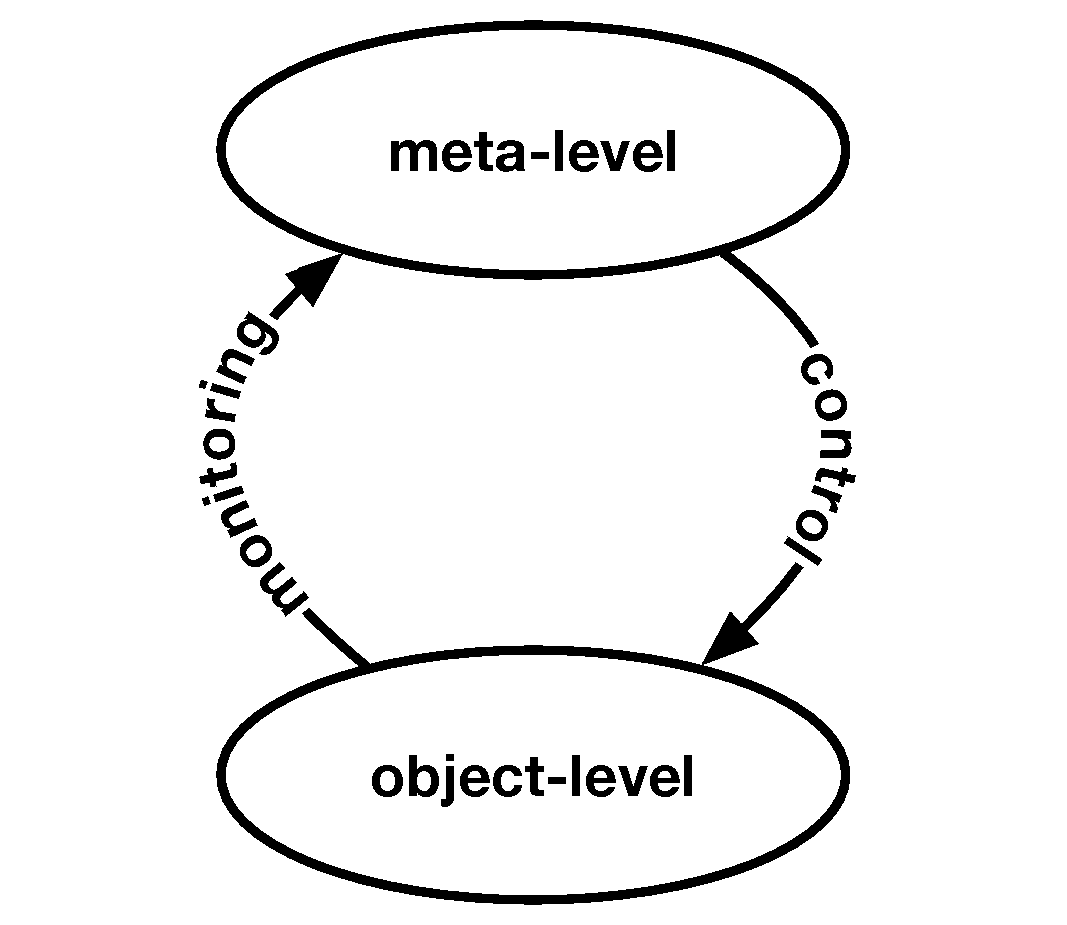
\includegraphics[width=0.4\textwidth]{figs/memory/nelson.pdf}
  \caption{\captiontitle{Illustration of Nelson and Narens' theoretical framework for metamemory.} A ``meta-level'' process monitors and controls the performance of a basic ``object-level'' process. Adapted from \citetnelson{}.}
  \label{fig:nelson}
\end{SCfigure}


\begin{figure}[ht]
  \centering
  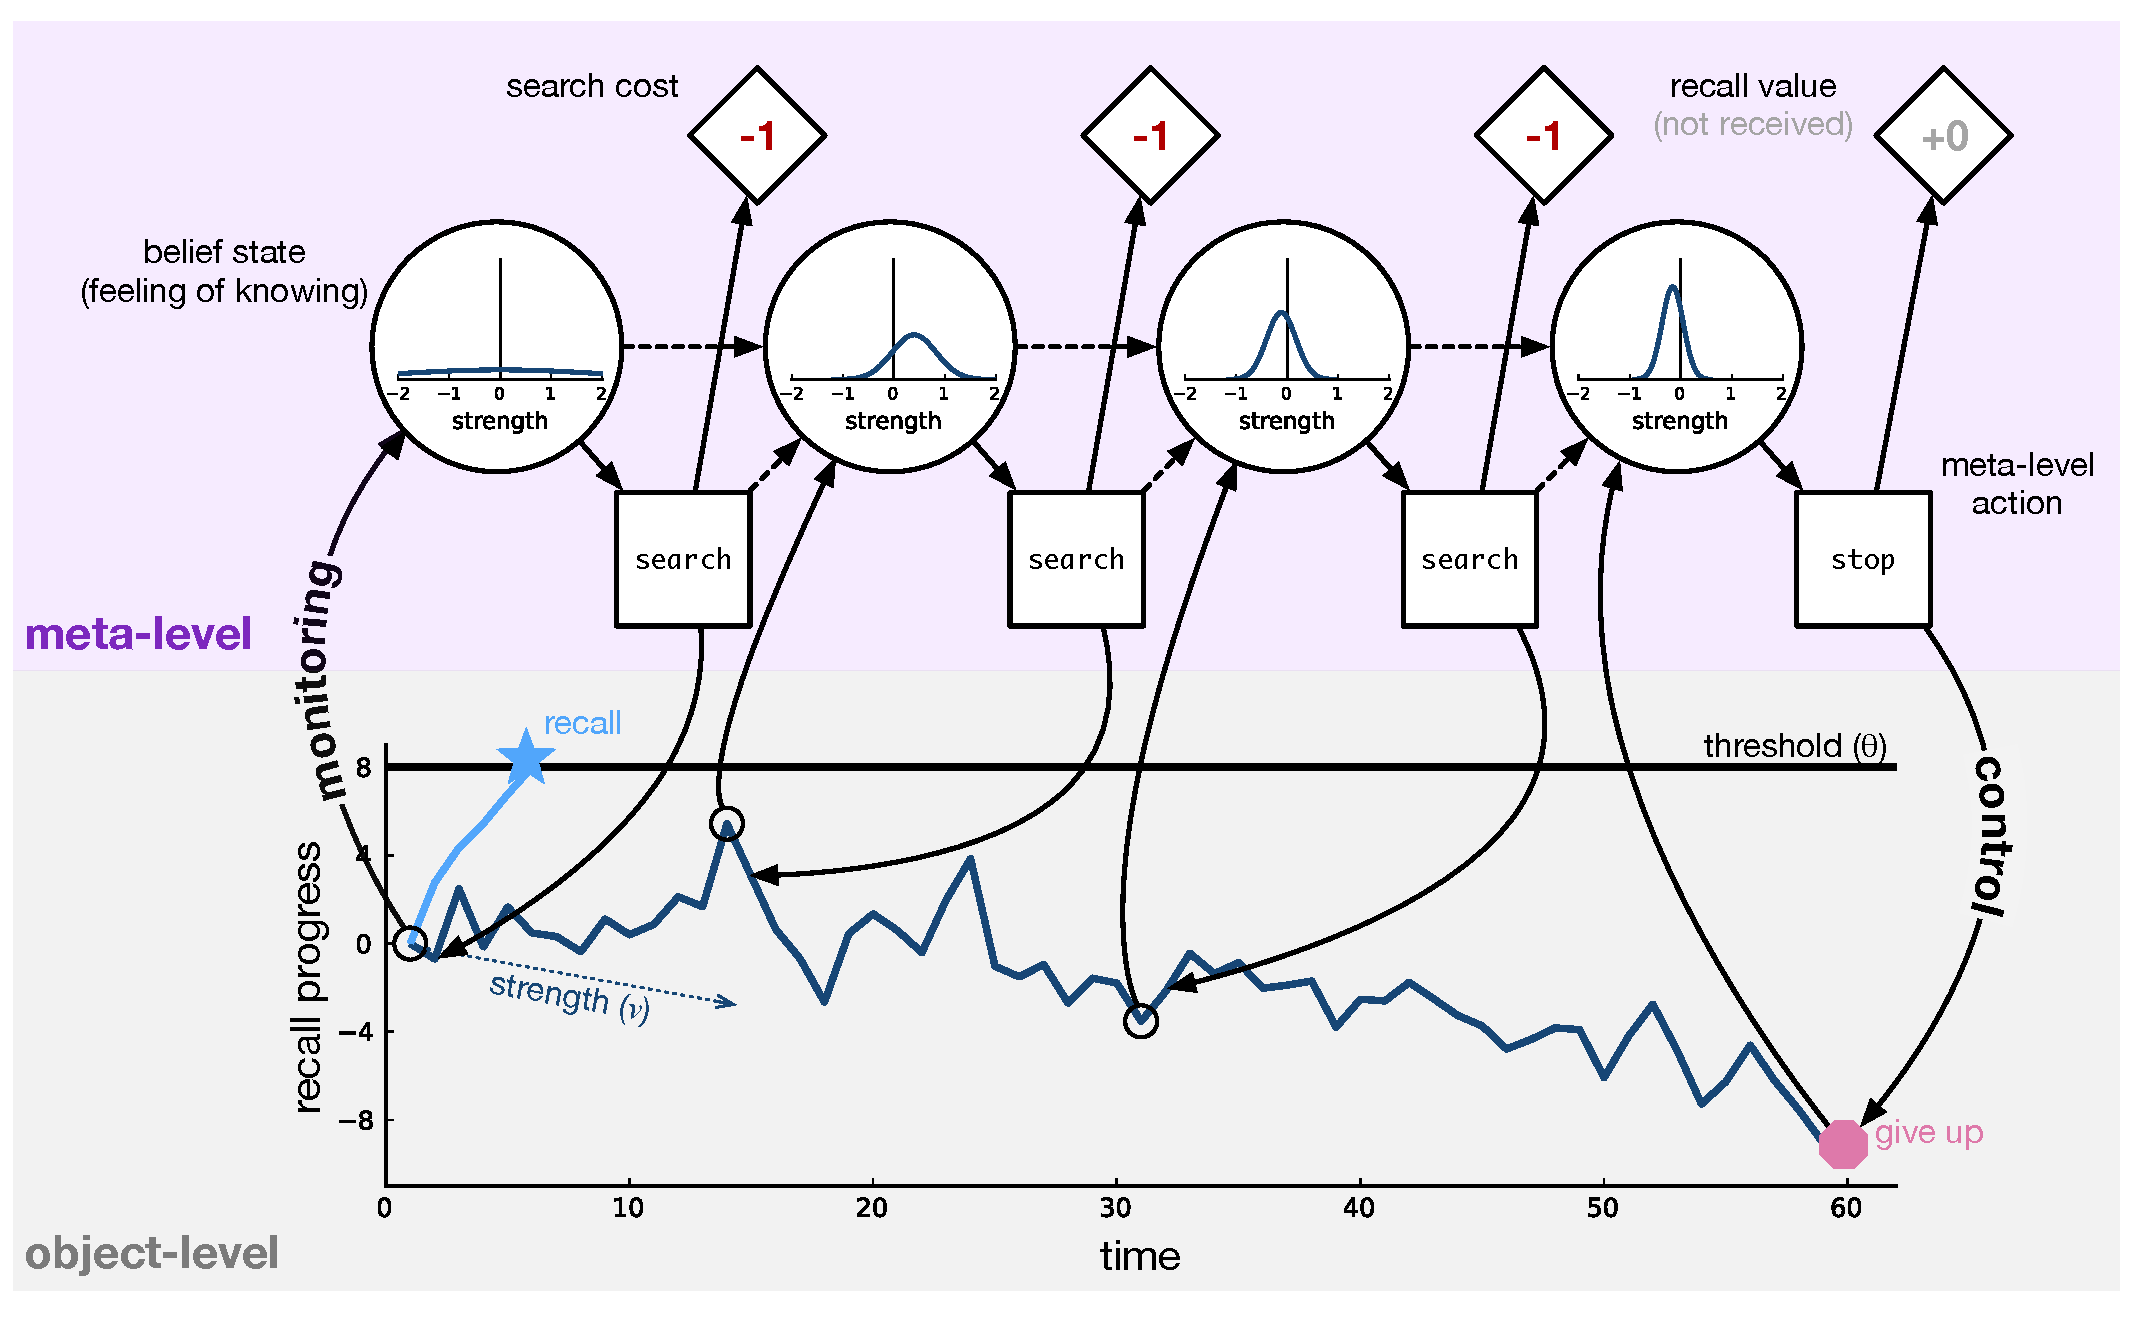
\includegraphics[width=\textwidth]{figs/memory/model.pdf}
  \caption{\captiontitle{A dynamic model of metamemory.}
    Bottom: The object-level recall process is modeled as evidence accumulation. A memory is recalled when a threshold level of evidence is accumulated, with the speed of accumulation (the drift rate) corresponding to the strength of the memory. Top: the meta-level process monitors and controls the object-level recall process. This is modeled as a Markov decision process (MDP) where the states (circles) correspond to beliefs about the memory's strength and the actions determine whether search continues; the rewards capture the cost of search and the cost of failing to retrieve a memory. Solving this MDP yields an optimal policy for determining when to stop searching memory based on partial recall progress.}
  \label{fig:model-diagram}
\end{figure}

\section{Empirical evidence for control in memory recall}

A number of behavioral studies have already suggested that people are capable of using their ability to monitor their memory in the service of controlling their memory processes. At the acquisition phase, a large body of work has investigated how people preferentially allocate study time depending on how well they have learned different pieces of information \citep{dunlosky1998training,metcalfe2009metacognitive,gureckis2012selfdirected}. Another substantial literature has addressed how people choose which memories to maintain or forget \citep{castel2007adaptive,williams2013benefit,suchow2016deciding,hu2019role}. Here, however, we focus specifically on the control of recall.

Most work on metamemory for recall boils down to one essential question: How do people decide whether to (continue to) search for a memory? The initial decision of whether or not to search at all is often treated as part of a more general \emph{strategy selection} process \citep{reder1988strategic}, with memory search being one of multiple possible strategies (along with, e.g., looking up the information in a dictionary). The choice of strategy appears to be driven by an initial feeling-of-knowing \citep{nhouyvanisvong1998rapid}, which is itself driven by surface-level properties of the question, such as familiarity with its terms \citep{reder1992determines}. A key finding from this line of work is that people can estimate the probability that they will be able to recall a target faster than they can actually recall it \citep{reder1987strategy}. This necessitates some form of metacognitive monitoring, as participants cannot be making judgments of recallability based on the outcome of recall if the former precedes the latter.

Once a memory search has been initiated, how long do people search before giving up? A key finding here is that participants spend longer before giving up on questions for which they report greater feeling of knowing \citep{nelson1984comparison,nhouyvanisvong1998rapid,gruneberg1977methodological,lachman1979metamemory} or being in a tip-of-the tongue state \citep{schwartz2001relation}. For the latter, participants also show worse performance on a secondary task, indicating more focused processing \citep{ryan1982motivated}. Feeling of knowing and tip-of-the tongue states are themselves associated with greater subjective familiarity \citep{reder1988strategic}, partial recall of the target \citep{brown1966tip,koriat1993how,schacter1985attribute} and the ability to recall given additional information \citep{gruneberg1974feeling}. Together, these results suggest that people are able to accurately identify targets they are likely to recall with further effort, and allocate that effort accordingly.

A related finding, although not one central to control, is that participants give higher confidence judgments when they recall an answer more quickly \citepnelson{}. In conjunction with the feeling-of-knowing effects, this produces a striking pattern. Treating both feeling of knowing and confidence as judgments of memory strength, we see opposite relationships between judged strength and response time for successful vs. failed recall. \citet{costermans1992confidence} demonstrated this pattern in a single study. On each trial, participants were given a general knowledge question. Then, if they provided an answer, they gave a confidence judgment; if they were unable to provide an answer, they instead gave a feeling-of-knowing judgment. Costermans et al. found that, on the recall trials, participants gave higher confidence judgments when they responded more quickly. But on the omission trials, participants gave higher feeling-of-knowing judgments when they responded more \emph{slowly}. In the following section, we will show that both of these findings are consistent with a model in which memory recall follows an evidence accumulation process and search is terminated optimally based on metacognitive monitoring of the rate of progress.

\section{An optimal model of metamemory for recall}

Following classic theories of metamemory (\citealpnelson{}; Figure~\ref{fig:nelson}), we specify our model as two interrelated processes operating at different levels. The \emph{object-level} process includes the mechanisms supporting recall itself. Here, we abstract away from the details of memory search, modeling recall instead as a simple evidence accumulation process \citep{ratcliff2002estimating,sederberg2008context}. The \emph{meta-level} process supervises the object-level process; it \emph{monitors} the rate of progress towards recall and \emph{controls} how long the search process is allowed to continue. Here, we assume that the meta-level process is optimal in the sense that it stops searching when the expected costs of search outweighs the expected benefits.

Importantly, we do not intend this model as a precise characterization of the mechanisms underlying human metamemory, nor do we hope to achieve a close quantitative fit to data. Instead, our goals are to (1) characterize the problem that a metamemory system must solve, and (2) identify qualitative behavioral signatures of a system that solves this problem well. This will allow us to determine in which ways people can or cannot deploy metamemory adaptively, potentially generating clues about the nature of the true underlying cognitive processes. The model is illustrated in Figure~\ref{fig:model-diagram}; we describe its components below.

\subsection{Object-level process}

We model recall as a process of evidence accumulation. Evidence accumulation (or ``sequential sampling'') models assume that decisions are made by accumulating noisy information over time until a threshold level of evidence is reached. They have been widely applied in the decision-making \citep{busemeyer1993decision,usher2001time,ditterich2006stochastic,krajbich2010visual} and memory \citep{ratcliff1978theory,sederberg2008context} literatures, and are successful in accounting for the effects of various experimental manipulations on accuracy and response times during recognition and recall tasks \citep{ratcliff2002estimating,sederberg2008context,yonelinas2010recollection}. In our model, the ``evidence'' captures progress towards recalling a target. Thus, when a threshold level of evidence is reached, the target is recalled (blue star in Figure~\ref{fig:model-diagram}).

Concretely, at each time point $t$, the current recall progress $z_t$ is incremented by a sample from a Gaussian distribution,
%
\begin{equation}\label{eq:evidence}
  z_t = z_{t-1} + x_t \,\text{ where }\,
  x_t \sim \mNormal{v, \sigma^2}.
\end{equation}
%
The mean of this distribution, $v$, controls the rate of accumulation; it is often called the \emph{drift rate} (illustrated as a thin dashed blue arrow in Figure~\ref{fig:model-diagram}). In our model, it captures the strength of the memory. The noise $\sigma^2$ captures the consistency of that progress. The target is recalled when the total progress exceeds a threshold $\theta$.

% It is worth noting that we view evidence accumulation as an abstraction of the true processes underlying memory recall. The key assumptions we make about the object-level process are that (1) recall progress is graded rather than all-or-none, and (2) early progress is at least somewhat indicative of the prospect for future progress. These assumptions are also made by verbal theories of metacognitive control in metamemory (e.g., \citealp{koriat2000control}), and are met by many process-level theories of memory recall, for example... 

\subsection{Meta-level process}
The problem of deciding when to cut off an unsuccessful memory search is addressed by the meta-level process. That is, the meta-level process \emph{controls} how long the object-level process is allowed to continue. How should it do so? From a rational perspective, one should keep searching as long as the probability of recall multiplied by the utility of recall is greater than the expected cost of search \citep{anderson1989human}. Putting this logic into notation, we can define the optimal meta-level action as
%
\begin{equation}\label{eq:anderson}
  a^* = \begin{cases}
    \search & \text{if } p\recall \cdot U\recall > \E [\text{cost}(\text{search})] \\
    \term & \text{otherwise}
  \end{cases}
\end{equation}
%
where $U$ stands for utility. The challenge lies in estimating $p\recall$ and $\E[\text{cost}(\text{search})]$. In our evidence-accumulation model, these values correspond respectively to the probability that the evidence will eventually cross the threshold and the time point at which this occurs. 

Intuitively, one could accurately estimate the probability and cost of future recall if one knew the strength of the target memory, $v$. However, a key assumption of our model---and the metamemory literature more broadly---is that the meta-level process does not have direct access to this information. Instead, we assume that the meta-level process must infer the memory's strength by \emph{monitoring} the object-level process. The existence of such a monitoring process is widely agreed on; however, its precise nature is controversial. In particular, it is unclear to what extent monitoring tracks the underlying memory strength \citep{hart1965memory}, partial recall progress \citep{koriat1993how}, or superficial cues that happen to be predictive of recall \citep{reder1992determines,schwartz1992cue}. Resolving this debate is beyond the scope of this paper. Thus, for simplicity and tractability, we assume that the meta-level process directly observes the state of the object-level process. We emphasize that this is purely a simplifying assumption, and not a claim about how people actually monitor their memory. We return to this point in the discussion.

Concretely, we assume that the meta-level process observes the current recall progress $z_t$ and the time spent so far $t$, which provides a complete summary statistic for the entire sequence up to time $t$. Given this information, the meta-level process then infers a posterior distribution over the strength of the memory,
%
\begin{equation}\label{eq:belief}
\begin{gathered}
  p(v \mid z_t, t) = \mNormal{v; \mu_t, \sigma_t^2} \\
  \mu_t = \frac{z_t t \sigma^{-2} + \mu_0 \sigma_0^{-2}}{\sigma_t^{-2}} 
  \quad\quad
  \sigma^2_t = \frac{1}{t \sigma^{-2} + \sigma_0^{-2}}
\end{gathered}
\end{equation}
%
where $\mu_0$ and $\sigma_0^2$ encode the agent's prior, $\mNormal{\mu_0, \sigma_0^2}$. To build intuition, note that with a very weak prior (large $\sigma_0^2$), $\mu_t$ reduces to $\nicefrac{z_t}{t}$, the average rate of recall progress. This time-varying belief about the strength of a memory formalizes the concept of \emph{feeling of knowing}.

Given this estimate of memory strength, how should the meta-level process determine whether to continue searching. That is, how should \emph{monitoring} inform \emph{control}? One intuitively appealing strategy is to estimate future recall progress by repeatedly applying Equation~\ref{eq:evidence}, compute $p\recall$ and $\E[\text{cost}(\text{search})]$ from those estimates, and then choose the optimal action by Equation~\ref{eq:anderson}. However, this strategy fails because it implicitly assumes that the object-level process will be allowed to continue indefinitely---precisely what the meta-level process is intended to prevent. The decision of whether to stop is not made just once; it is continually remade at each time step. As a result, the probability and cost of recall---and therefore the optimal stopping decision---depend on one's future stopping decisions.

Thus, we see that metamemory poses a particularly thorny type of decision problem, one where one's current choice depends on one's future choices. That is, metamemory poses a \emph{sequential decision problem}. Fortunately, a great deal of work in artificial intelligence has focused on solving exactly this sort of problem, typically using the formalism of \emph{Markov decision processes} (MDPs). An MDP is defined by a set of states the environment can be in $\S$, a set of actions the agent can take $\A$, a transition function specifying how actions change state $T$, and a reward function specifying the agent's goals $r$. MDPs are the key formalism underlying reinforcement learning \citep{sutton2018reinforcement}, supporting recent advances in artificial intelligence \citep{mnih2015human,silver2017mastering} as well as providing a foundation for the psychology and neuroscience of decision-making \citep{niv2009reinforcement,dayan2008decision,glimcher2011understanding}.

The insight that meta-level control poses a sequential decision problem has been formalized by the field of rational metareasoning \citep{russell1991principles}, which has the goal of building artificial intelligence that makes efficient use of their limited computational hardware. In particular, we apply the framework of \emph{meta-level Markov decision processes} \citep{hay2012selecting}, which models the meta-level control problem as an MDP. In a meta-level MDP, the states correspond to beliefs about the world and the actions correspond to computations (or cognitive operations) the agent can execute. The transition function describes how computations update beliefs, and the reward function encodes the cost of computation as well as the benefits of acting according to a more refined belief.

In our meta-level MDP model, a state $s \in \S$ captures both the current recall progress as well as the belief about memory strength (feeling of knowing). Because the belief depends only on the recall progress and time spent so far (Equation~\ref{eq:belief}), the state can be compactly represented as $s_t = (t, z_t)$. There are two possible actions $a \in \A$: $\search$ continues searching for the memory and $\term$ terminates recall. 

The reward function $r$ encodes the benefit of recall and the cost of search:
\begin{equation}\label{eq:reward}
  r(s_t, a_t) = \begin{cases} 
    U\recall & \text{ if } z_t \geq \theta \\
    -\samplecost & \text{ if } a_t = \search \\
    0 & \text{ if } a_t = \term.
  \end{cases}
\end{equation}
where $U\recall$ specifies the utility of correct recall (capturing, in our case, experimental incentives) and $\samplecost$ is a free parameters that specifies the cost of searching for one time step (capturing any experimentally imposed costs as well as implicit costs such as the opportunity cost of the time spent searching).

Finally, the transition function $T$ captures the dynamics of the object-level process: the fact that $\term$ terminates the process, and (implicitly) the Bayesian belief updating. Note, however, that the object-level dynamics depend on the true memory strength ($v$ in Equation~\ref{eq:evidence}), which the agent does not have access to. Thus, the transition function must marginalize over the strength according to the current belief state:
%
\begin{equation}\label{eq:mem-transition}
\begin{aligned}
  % T(s_{t+1} | s_t, a) = \int p(z_{t+1} \mid z_t, v)p(v \mid z_t, t) \ dv
  T(s_{t+1} | s_t, a) 
  &= p(z_{t+1} \mid t, z_t) \\
  &= \int p(z_{t+1} \mid z_t, v) p(v \mid t, z_t) \ dv \\
  &= \int \mNormal{z_{t+1} - z_t \mid v, \sigma^2} 
          \mNormal{v \mid \mu_t, \sigma_t^2}\ dv \\
  &= \mNormal{z_{t+1} - z_t \mid \mu_t, \sigma^2 + \sigma_t^2}.
\end{aligned}
\end{equation}
%
The two substitutions in the third line follow from Equations~\ref{eq:evidence} and~\ref{eq:belief}, respectively. The final line is a standard property of Gaussian distributions \citep{murphy2007conjugate}.


\subsection{Optimal policy}

We have now defined a meta-level MDP that formalizes the problem of deciding when to give up on recalling a memory. The final step is to specify a strategy for solving that problem. In MDP terms, we need to specify a policy $\pi$ that chooses which action to take in each state. Here, we focus on the optimal policy, which is the one that maximizes the total expected reward. As detailed in the methods, we can identify this policy by computing the optimal value function $V^*$, which specifies the maximal total reward one could expect to gain starting from any given state. To build intuition, we can factorize $V^*$ for the current model into two components, capturing the utility of recall and the cost of search,
%
\begin{equation}\label{eq:value}
  V^*(s_t) = p(\text{recall} \mid s_t) U\recall - 
  (\E\left[t_\text{max}\mid s_t\right] - t)\samplecost,
\end{equation}
%
where $t_\text{max}$ is the time step on which the item is recalled or the search is terminated. The optimal policy is then defined as
%
\begin{equation}\label{eq:policy}
  \pi^*(s_t) = \begin{cases}
    \search & \text{if } \E_{s_{t+1} \sim T(\cdot \mid s_t, \search)}[V^*(s_{t+1})] > \samplecost \\
    \term & \text{otherwise}
  \end{cases}
\end{equation}
%
To understand this equation in comparison to Equation~\ref{eq:anderson}, note that $p\recall$ and $\text{cost}(\text{search})$ have each been split into two components, capturing immediate versus future outcomes. The immediate recall probability is encoded in the transition function, $T(\cdot \mid s_t, \search)$; the immediate search cost is encoded in the reward, $-\samplecost$. The expected future outcomes are both integrated into $V^*(s_{t+1})$, as shown in Equation~\ref{eq:value}.
% Critically, $V^*(s_{t+1})$ is itself defined in terms of $\pi^*(s_{t+1})$, capturing the aforementioned sequential dependence between current and future stopping decisions.
A key advantage of specifying our model as an MDP is that we can apply standard techniques (in particular, backwards induction) to compute $V^*$, allowing us to identify an optimal policy for metamemory. See the Methods below for details.


\begin{figure}[ht]
  \centering
  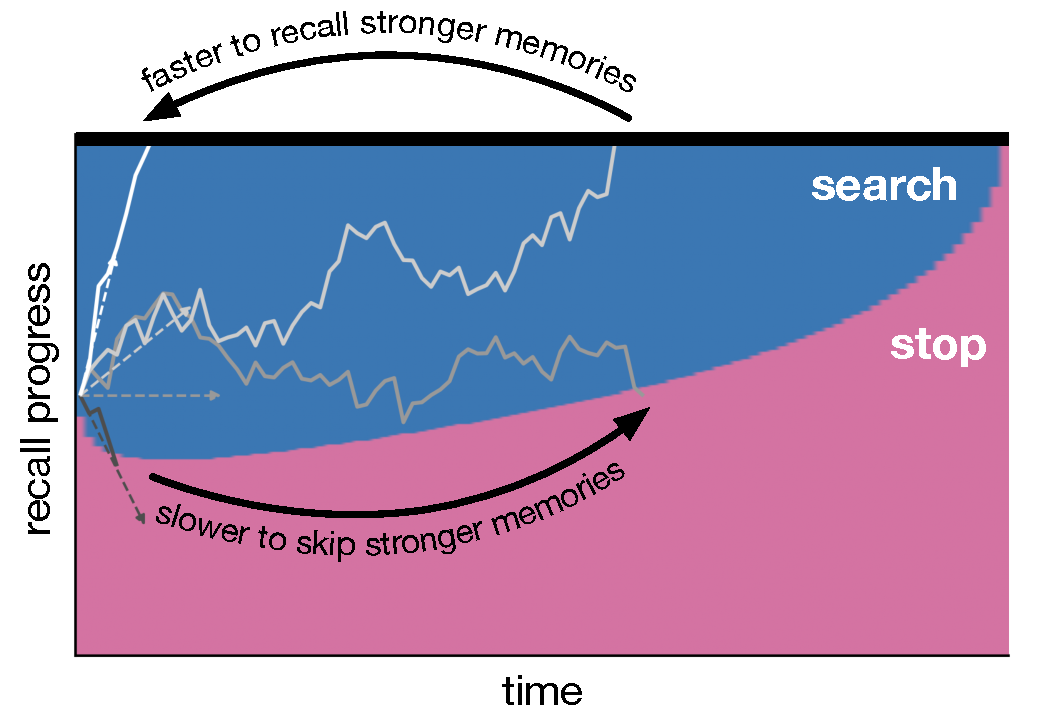
\includegraphics[scale=0.45]{figs/memory/exp1_predictions.pdf}
  \caption{\captiontitle{Experiment 1 optimal policy and predictions.}
    The optimal policy partitions the state space into two sections, one (blue) in which the policy continues searching, and another (pink) in which it terminates search. The response time for each trial is thus given by the first time point at which the recall progress either exceeds the threshold (recall) or enters the pink region (no recall). In the former case, stronger memories (lighter lines) will result in faster responses because such memories accumulate progress and hit the threshold faster. In the latter case, stronger memories will result in slower responses because such memories can hover in the search region before ultimately hitting the stop region.
  }
  \label{fig:exp1_predictions}
\end{figure}

\subsection{Predictions}

As illustrated in Figure~\ref{fig:exp1_predictions}, the model makes two key predictions regarding the relationship between memory strength and response time. First, stronger memories should be recalled more quickly because stronger memories accumulate progress faster and hit the threshold sooner. Note that this prediction is a simple consequence of the object-level process and does not depend on metacognition. Second, stronger memories should be abandoned less quickly. In particular, while the meta-level process can quickly identify very weak memories as such (leading it to terminate search), marginal-strength memories produce ambiguous evidence and it takes more time for the meta-level process to determine that the memory is too weak to justify further search.

Figure~\ref{fig:exp1_predictions} also highlights that the optimal policy can be represented as a time-varying threshold, such that search is terminated if the progress ever falls below the threshold (c.f. \citealp{drugowitsch2012cost}). In the language of \citet{marr1982vision}, this can be understood as an algorithmic-level implementation of the computational-level theory outlined above. We return to this point in the General Discussion. Note that the threshold is non-monotonic because a fixed amount of negative progress provides stronger evidence that the memory has low strength if the negative progress was generated more quickly.

\begin{figure}[htb!]
  \centering
  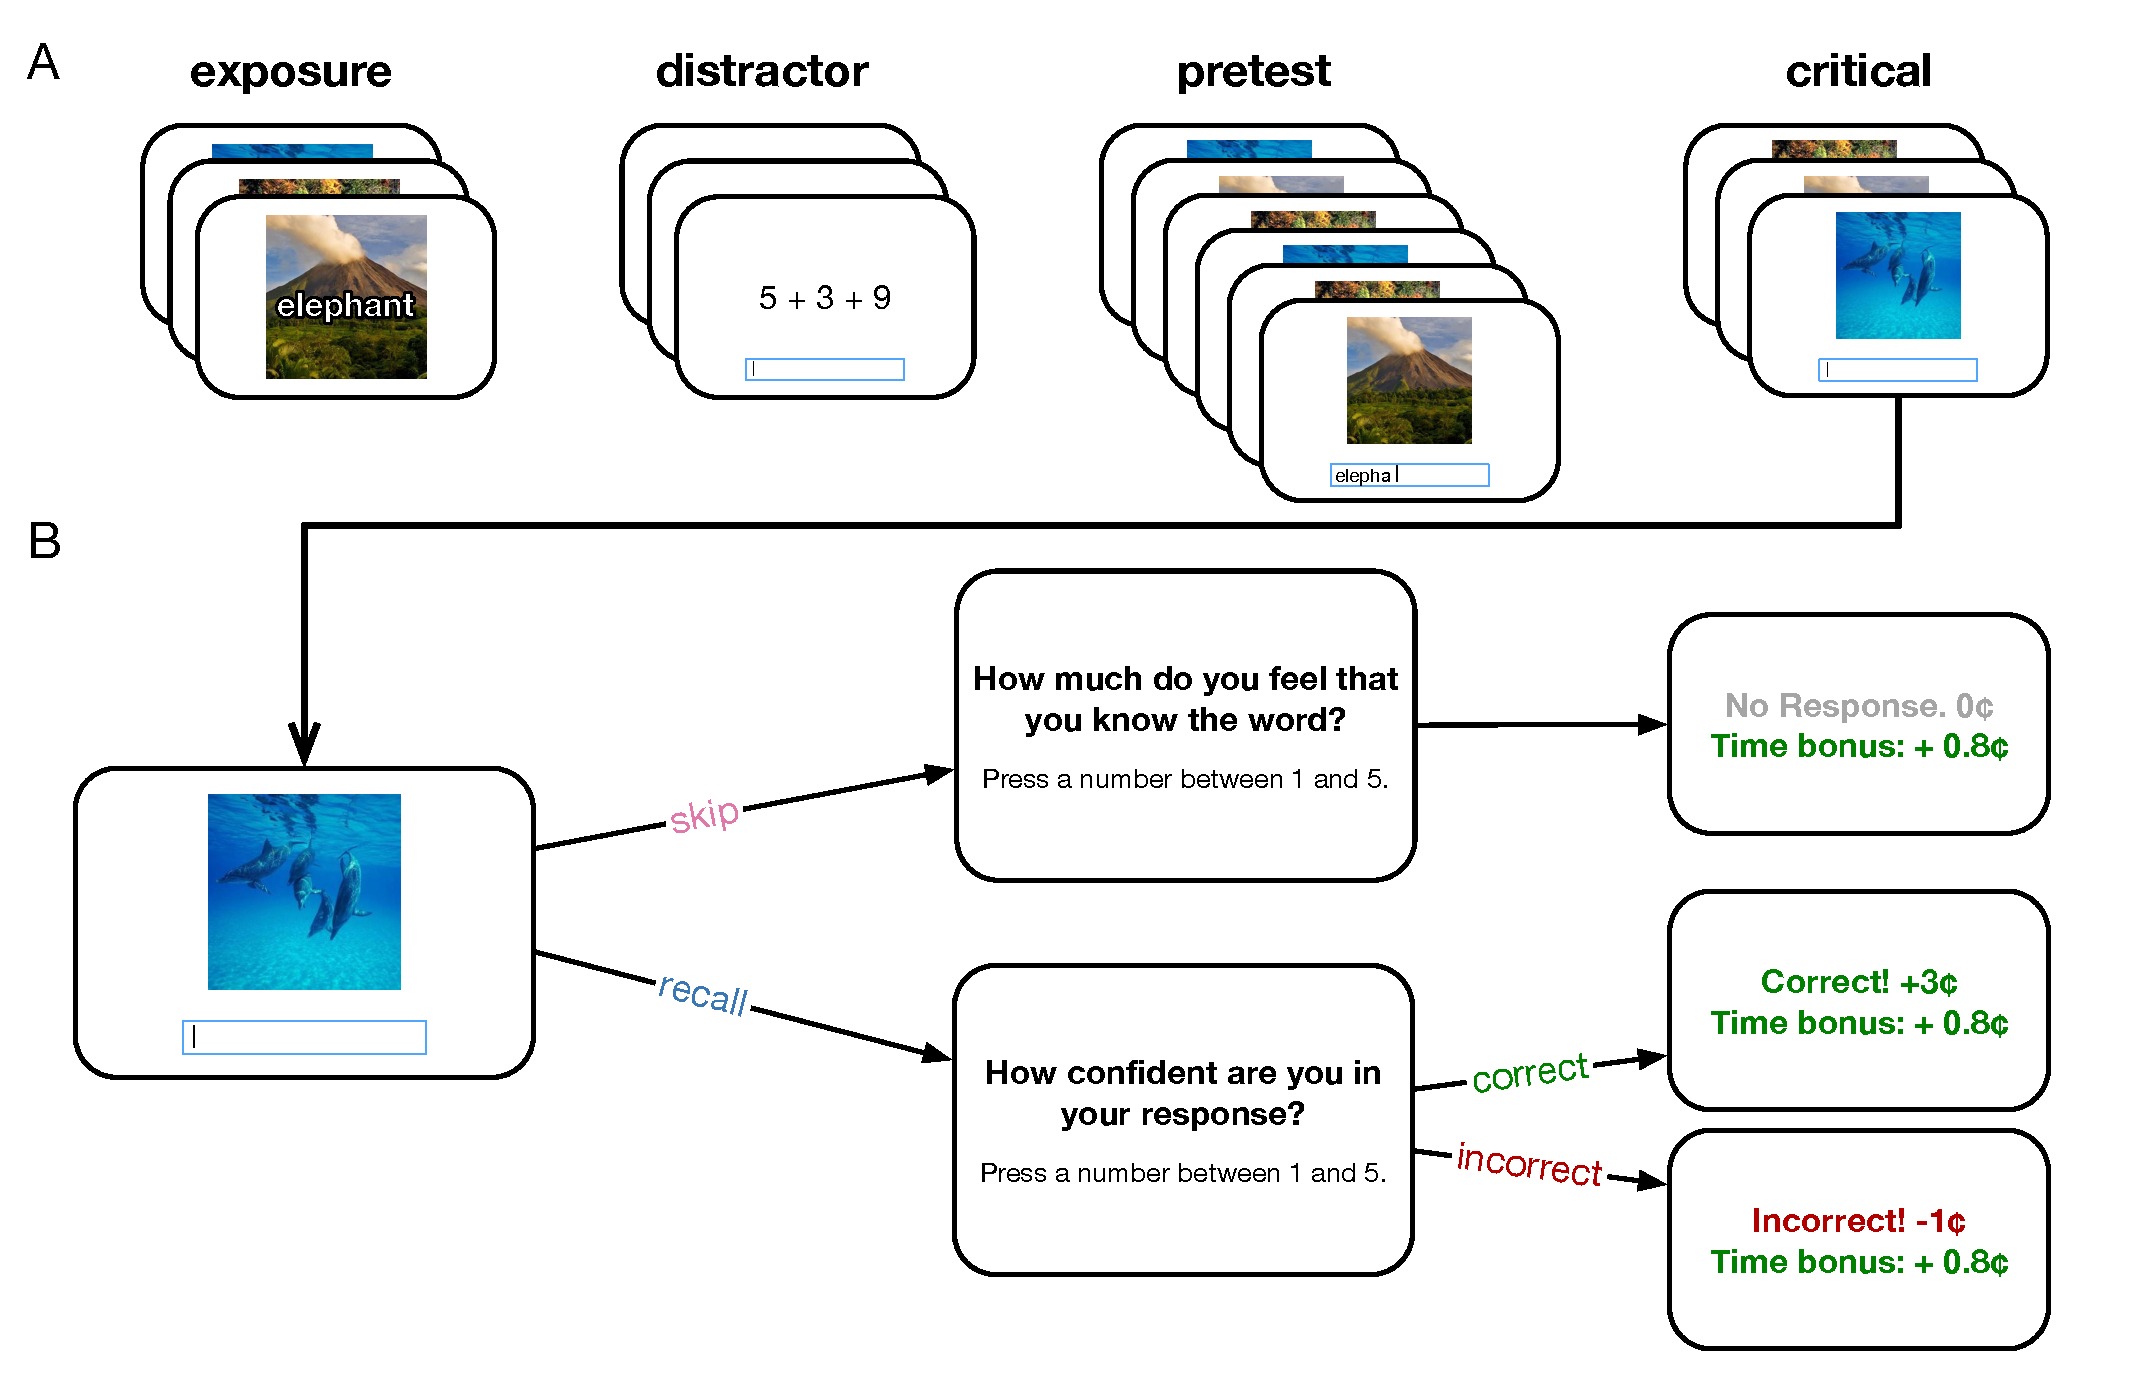
\includegraphics[width=\textwidth]{figs/memory/task_exp1.pdf}
  \caption{\captiontitle{Experiment 1 procedure.} 
    \subcap{A} Participants viewed 40 image-word pairs for two seconds each (exposure). They then completed simple math problems for 60 seconds (distractor). Next, they attempted to recall the word associated with each image, two trials per image (pretest). Finally, they completed one critical trial for each image.
    \subcap{B} Critical trials were similar to pretest trials, except that incorrect responses were penalized. The penalty could be avoided by providing an empty response, ``skipping'' the trial. After giving a response, participants made a metamemory judgment, confidence if they had entered a word and feeling-of-knowing if they had not. A speed bonus was given regardless of the response.}
  \label{fig:task-exp1}
\end{figure}

\section{Experiment 1}

In our first experiment, we sought to replicate and extend the findings of \citet{costermans1992confidence} in a cued-recall setting (Figure~\ref{fig:task-exp1}). The key finding from the original study was that participants reported higher confidence judgments on trials where they more quickly recalled the answer to a question, but lower feeling-of-knowing judgments when they more quickly reported being unable to recall the answer. Our model can capture both of these effects under the assumption that the metamemory judgments are based on the inferred memory strength at response time (explained below). However, it is also possible that the metamemory judgments reflect a purely post-hoc rationalization of the longer response time, not influencing the decision to stop at all. To rule out (or at least cast doubt on) this explanation, we modified the task such that we could obtain objective measures of memory strength before the critical trials. Specifically, we used a cued-recall paradigm that allowed us to query the same target multiple times. This allowed us to test whether people's stopping decisions depended on their true memory strength, as the optimal policy predicts they should.

\subsection{Methods}

All sample sizes, exclusion criteria, statistical analyses, modeling procedures, and plotting decisions were pre-registered. After pre-registering, we discovered a conceptual error in our implementation of a lesioned model. The corrected model was able to capture some results we believed were specific to the main model; we thus omitted those results. See Appendix~\ref{app:deviation} for details, including the omitted results.

\subsubsection{Participants}

We recruited 612 participants through Prolific with the restriction that they reported current U.S. or U.K. residence, had at least a 95\% approval rating, and had not participated in any pilot studies. As pre-registered, we excluded 106 participants who did not provide a response on more than 90\% of critical trials. This yielded 506 participants in our final analysis. The target sample size of 500 participants had over 95\% power based on a boot-strapping power analysis conducted on pilot data.

\subsubsection{Stimuli}

Each participant was randomly assigned 40 images and words, which were arbitrarily paired. The images were randomly sampled from 40 common scene categories (one image per category), selected from the Scene UNderstanding (SUN) database (\citealt{5539970}). We manually removed photos that contained a person. All images were resized and then cropped to 300 by 300 pixels. The words were selected randomly from those used in \citet{madan2021exploring}, which were themselves selected from the University of South Florida free association norms word database \citep{nelson2004university}.

\subsubsection{Procedure}

The experiment consisted of four phases: exposure, distractor, pretest, and critical. After learning the mapping between images and words through a single round of passive exposure, participants solved simple arithmetic problems to clear working memory. They then completed the pretest and critical trials, both of which involved cued recall. In the pretest trials, participants were given an image and asked to type in the corresponding word; they were incentivized to be both accurate and fast. These trials provide an objective measure of how well each participant had learned each pair. In the critical trials, we increased the speed incentive and added an error penalty. However, we also allowed participants to skip a trial without penalty, still earning the speed bonus. This creates an incentive to quickly identify trials in which the target is unlikely to be correctly recalled. We provide further details on the procedure for each of these components below.

\paragraph{Exposure} On each exposure trial, participants viewed a word superimposed on the center of an image; the word was printed in white font with black outlines such that it would be clearly legible on any image. The pair was shown for two seconds, with a half-second inter-trial interval. Each of the 40 pairs was shown once.

\paragraph{Distractor} On each distractor trial, a simple arithmetic problem was presented and participants had three seconds to enter the correct answer. Each problem was an addition of three single-digit numbers. After a response (or timeout), feedback was presented for at least one second. If a response was made before the deadline, the feedback phase was extended such that all trials lasted exactly four seconds. Participants were informed that they would earn one cent for each correct answer. Due to a programming error, participants were incorrectly instructed that they would have five seconds to enter a response; however, no participant reported noticing this discrepancy in the debriefing survey.

\paragraph{Pretest} Each pretest trial began with a blank screen and the text ``press space when ready.'' When the participant pressed space, an image, text box, and timer appeared. The timer immediately began counting down from 15 seconds. The trial ended when the participant entered a word (by typing it into the text box and pressing enter) or when the timer expired. If the timer expired, ``Timeout'' appeared in large red letters. No other trial-by-trial feedback was provided. Participants were instructed that they would receive one cent for each correct answer, as well as a small extra bonus for answering quickly and correctly. (The time bonus was a quarter of a cent multiplied by the proportion of time left when a response was given). At the end of each block, participants received a summary of their performance, separately indicating the amount of bonus money they made from correct responses and from response speed. There were two blocks, and each image was shown once in each block, for a total of 80 trials. The first trial in the first block was a practice trial and was excluded from analysis.

% cite http://memory.psych.upenn.edu/files/pubs/KahaEtal02.pdf

\paragraph{Critical trials} The critical trials were similar to the pretest trials, but with a different incentive scheme. The bonus for correct responses was increased to three cents, but a one-cent penalty for incorrect responses was introduced. Additionally, participants could skip a trial by pressing enter without typing a word; this did not incur a penalty. Finally, the speed incentive was raised to a tenth of a cent for each second left on the timer (i.e., up to 1.5 cents per trial). The speed bonus was given on all trials, including skip and error trials. To ensure that participants understood the incentives, they were required to pass a quiz, affirming that there was a penalty for mistakes, no penalty for skipping, and a time bonus regardless of response type. Participants were additionally encouraged to quickly skip trials for which they didn't know the word.

After a response was given, a metamemory judgment was elicited. When participants gave a response, they were asked ``how confident are you in your response?'' They then pressed a number between 1 and 5 to indicate that they were ``not at all sure'', ``not so sure'', ``more or less sure'', ``nearly sure'', or ``absolutely sure'' their response was correct. If they did not give a response (i.e., they skipped the trial), they were asked ``how much do you feel that you know the word?'', again pressing a number between 1 and 5. The responses were described as: ``I am absolutely sure I do not know the word', ``I am rather sure I do not know the word', ``I have a vague impression I know the word', ``I am rather sure I know the word' and ``I am absolutely sure I know the word.'' 

\begin{figure}[t!]
  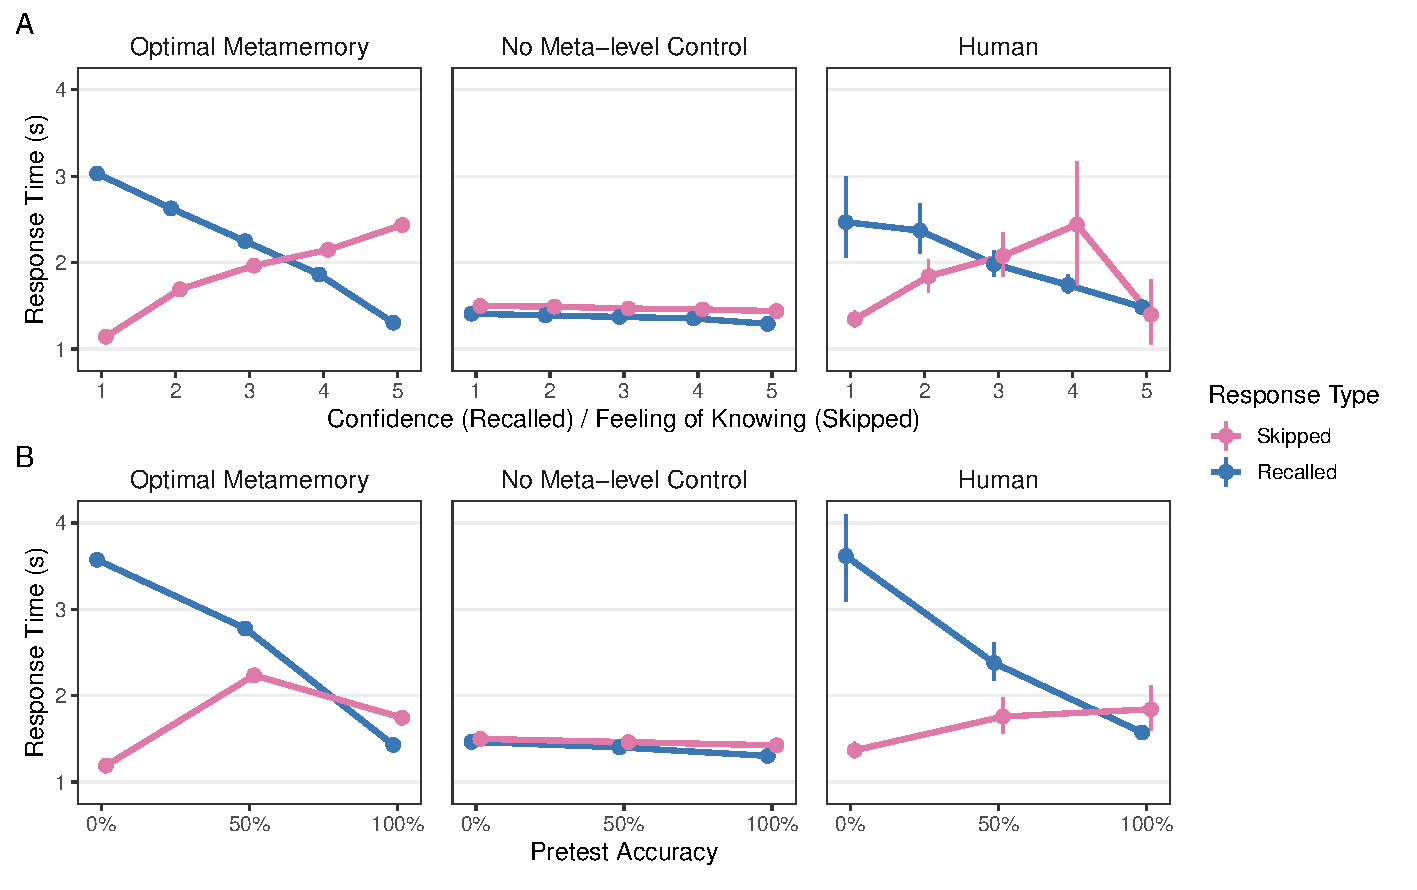
\includegraphics[scale=.65]{figs/memory/exp1/rt.pdf}
  \caption{%
    \captiontitle{Opposing effects of memory strength on time to recall vs. skip a target.}
    \subcap{A} Reaction time as a function of metamemory judgment (feeling of knowing for skip trials, confidence for recall trials), separately for trials in which participants correctly recalled the target vs. skipped without responding (errors are excluded). The left panel shows the predictions of the proposed optimal metamemory model, the center panel shows the predictions of a model with the same recall process but no meta-level control (sampling stopping time from the empirical distribution), and the right panel shows human data. The models' metamemory judgments are made based on the inferred memory strength at the end of the trial.
    \subcap{B} The same, but as a function of accuracy rate for the presented cue in the pretest phase. 
    \emph{Note}: Points show means of participant medians and error bars show 95\% bootstrapped confidence intervals over participant medians. Each model is treated as one participant (with one million simulated trials). All plotting decisions (including which effects to show, the aggregation method, and axis limits) were pre-registered.
  }
  \label{fig:exp1_rt}
\end{figure}

\subsubsection{Modeling}

\paragraph{Computing the optimal policy}

We compute the optimal policy by backwards induction. See \citet{puterman2014markov} for a general description of the method; here, we report the details necessary to apply the method to our model.

Recall that a belief state in the model is a tuple $(z_t, t)$. Because backwards induction can only be applied in finite state spaces, we begin by discretizing the first dimension of the belief into 100 equally sized bins, ranging from $-\theta$ to $\theta$. Note that $\theta$ is the maximum possible value $z_t$ can take. The lower bound of $-\theta$ is an arbitrary choice; we found that the optimal policy for well-fitting parameters always terminated well before this value was reached (e.g., Figure~\ref{fig:exp1_predictions}), suggesting that this imposed lower bound did not meaningfully affect the solution.

We first computed the transition function. To account for the discretization, we computed the probability of transitioning from $(t, z_t)$ to $(t+1, z_{t+1})$ as $\Pr(a < z_{t+1} < b \mid t, z_t)$ where $a$ and $b$ are the boundaries of the bin with $z_{t+1}$ in the center. Because $z_{t+1}|t,z_t$ is Gaussian (Equation~\ref{eq:mem-transition}), we could compute this quantity with standard statistical library functions (the Normal CDF). For most bins, the boundaries were $z_{t+1} \pm \nicefrac{\theta}{100}$. The top bin was clipped at $b = \theta$ and the bottom bin was unbounded, with $a = -\infty$. This ensures that the transition probability from each state sums to one.

Next, we initialized the value function for all terminal belief states. The value of states with $z_t = \theta$ is $U\recall$ and the value of states with $t=150$ (the maximum trial duration) but $z_t < \theta$ is 0. Then, we iterated backward in time, computing the value of all states with $t=149$ as the maximum of the expected value of each possible action
%
\begin{equation}
\begin{aligned}
  V^*(s) = \max_{a \in \{\search, \term\}} Q^*(s, a) 
\end{aligned}
\end{equation}
where
%
\begin{equation}
  Q^*(s, \search) = \sum_{z_{t+1}} p(z_{t+1} | t, z_t) V^*(t+1, z_{t+1}) - \samplecost
\end{equation}
%
and $Q^*(s, \term) = 0$. The iteration continues with $t=148$ down to $t=1$. After computing $Q^*$ for all states and actions, the optimal action in each state can be quickly identified as
%
\begin{equation}
  \pi^*(s) = \argmax_{a \in \{\search, \term\}} Q^*(s, a) 
\end{equation}
%

\paragraph{Simulation procedure}
In order to compare the behavior of the model with that of our participants, we simulated experimental data. Simulating a trial corresponds to executing one ``episode'' of the meta-level MDP. That is, we initialized the state at $s_0 = (t=0, z_t = 0)$ and then repeatedly applied Equation~\ref{eq:evidence} to generate a sequence of states.\footnote{Note that we simulate data conditional on a known strength $v$ rather than with the transition function that marginalizes over $v$. This allows us to model multiple trials for a single cue/target pair, as described below.} At each time step, we first checked if the recall threshold has been exceeded, i.e. if $z_t > \theta$. If so, the episode ended and the trial was classified as a recall trial. Otherwise, we determined the optimal action $\pi^*(s_t)$, defined in Equation~\ref{eq:policy}. If the optimal action was $\term$, then the episode ended and the trial was classified as a skip trial. Otherwise, we repeated the process, unless the maximum time step had been reached, in which case the episode ended as a skip trial.

The simulated response time was determined based on the final value of $t$. We assumed that response times reflected both time spent actively searching memory as well as ``non-decision time'' spent on e.g., perceptually encoding the cue and preparing the motor response. For search time, we assumed that each time step took a fixed amount of time, a value we arbitrarily set to 100ms (the predictions of the model do not depend critically on this parameter; we chose 100ms to balance prediction fidelity with model runtime). For non-decision time, we assumed that it was drawn separately for each trial from a Gamma distribution, with parameters fit to data as described below. The simulated response time was the sum of the two components. Note that, for computational reasons, we did not factor the non-decision time into the timeout condition (the maximum timestep of 150 is the maximum trial duration of 15s divided by 100ms). This has a negligible effect on model predictions because timeouts were rare (less than 0.01\% of trials) with well-fitting parameter values.

The simulated metamemory judgments (confidence and feeling of knowing) were determined based on the posterior mean $\mu_t$ at the final time step, that is, when the target was recalled or the policy terminated search. To account for factors contributing to the judgment besides those captured by our model (e.g., individual differences in scale usage) we first corrupted $\mu_t$ with Gaussian noise, arbitrarily setting the variance to $\nicefrac{\sigma}{2}$. We then binned the continuous measure into five bins, corresponding to the 1-5 response scale. We set the bin boundaries separately for each judgment type in order to match the proportion of each response in the human data.

In order to capture the relationship between performance in the pretest and critical trials, we simulated both phases using the following procedure. For each simulated word/image pair, we sampled its memory strength $v$ from the prior distribution $\mNormal{\mu_0, \sigma_0^2}$. The parameters of the prior are free parameters of the model. Next, we simulated the two pretest trials for that pair by rolling out two episodes of the meta-level MDP. For these trials, we set $U\recall$ to the experimentally imposed value of one cent. The search cost $\samplecost$ is a free parameter. We then simulated the critical trial for the pair, setting $U\recall$ to the new value of three cents and increasing $\samplecost$ by the experimentally imposed value of 0.01 cents per sample (0.1 cents per second and 100ms per sample).

\paragraph{Parameter estimation}

The model's behavior is governed by six free parameters: the prior mean and standard deviation, $\mu_0$ and $\sigma_0$, the progress noise $\sigma$, the search cost $\samplecost$, and the mean and shape of the non-decision time (NDT) distribution, $\mu_\text{NDT}$ and $\alpha_\text{NDT}$.\footnote{%
  We use this parameterization rather than the traditional shape-scale parameterization to aid interpretability. The mean is the scale parameter multiplied by the shape parameter.
} We set these parameters by maximizing the likelihood of the critical trials at the group level. For fitting, we disregarded the metamemory judgment. Each trial (human or simulated) was thus defined by a pretest accuracy rate (0\%, 50\%, or 100\%), a response type (skip or recall), and a response time (discretized into 100ms bins from 0ms to 15000ms). 

Because the optimal policy does not depend on the the NDT parameters, we treated these separately (described below). For the remaining four parameters, we considered 50,000 configurations sampled pseudo-randomly according to the Sobol sequence \citep{sobol1967distribution,bergstra2012random} within the range ($\mu_0 \in (-0.5, 0.5),\ \sigma_0 \in (0, 1),\ \sigma \in (0, 1),\ \samplecost \in (0, 0.05)$). For each configuration, we computed the optimal policy by backwards induction, and then simulated 100,000 critical trials. For each simulated dataset, we constructed a $3 \times 2 \times 151$ histogram over possible trials (3 accuracy rates, 2 response types, and 151 response time bins). To apply the NDT model, we convolved this histogram with a Gamma distribution parameterized by $\mu_\text{NDT}$ and $\alpha_\text{NDT}$. Finally, to ensure non-zero probability was assigned to all trials, we mixed the model-predicted distribution with a uniform distribution with weight $10^{-6}$. The likelihood of each trial in the human dataset is simply the corresponding entry of this histogram. The total log likelihood is the sum of the log-likelihood for each trial.

Note that the NDT-convolution step does not require simulating the model. We thus optimized the NDT parameters for each configuration of the other four parameters using the Nelder Mead algorithm \citep{nelder1965simplex}. This provides the best possible likelihood for each configuration of the four primary parameters. We then selected the top 5000 such configurations, and approximated the likelihood more precisely, using 1,000,000 simulated trials. The best-performing configuration from this smaller set was then identified as the maximum likelihood estimate (MLE). The MLE was (\(
            \mu_0 = -0.002,\ 
            \sigma_0 = 0.186,\ 
            \sigma = 0.139,\ 
            \samplecost = 0.014,\ 
            \mu_\text{NDT} = 711.99,\ 
            \alpha_\text{NDT} = 8.87
        \)) with negative log-likelihood 70911. Note, however, that this exact number is arbitrary because it depends on the coarseness of the response time discretization.

\paragraph{Lesioned model without meta-level control}

In order to distinguish between model predictions that depend only on the object-level process vs. those that reflect adaptive meta-level control, we implemented a lesioned version of the model that lacks the control component. In this model, the decision to stop searching is no longer made by the optimal policy; instead, it is made randomly. Concretely, when simulating a trial from this model, we begin by sampling the stopping time from a Gamma distribution. We then apply Equation~\ref{eq:evidence} until either (1) the threshold is crossed, resulting in a correct trial as in the optimal model, or (2) the pre-determined stopping time is reached, resulting in a skip trial. This model has all the parameters of the main model except $\samplecost$, which only influences the optimal policy. It has two additional parameters for the stopping time distribution.

The parameters are fit by maximum likelihood estimation using the procedure described above. The MLE was \(
            \mu_0 = 0.201,\ 
            \sigma_0 = 0.326,\ 
            \sigma = 0.021,\ 
            \mu_\text{stop} = 289.0,\ 
            \alpha_\text{stop} = 22.67,\ 
            \mu_\text{NDT} = 1261.09,\ 
            \alpha_\text{NDT} = 2.03
        \) with negative-log likelihood 75083. We also considered a version of the model that samples stopping times directly from the empirical distribution. This model fit the data worse (negative log-likelihood of 77536; see Appendix~\ref{app:deviation}).

% We found that the maximum likelihood estimate for this model assigned very large values to the $\alpha_\text{NDT}$ and $\theta_\text{NDT}$, such that non-decision time accounted for about 77\% of the overall response time. As a result, the model predicted almost no effect of pretest accuracy on response times. Thus, to better visualize the behavior of the object-level process without meta-level control, we fixed the non-decision time parameters to the maximum likelihood estimate in the optimal model. We also considered models in which fixation durations were drawn directly from the empirical distribution, or with a Gamma distribution fit to the empirical distribution. None of these models captured the key behavioral pattern. See Appendix~\ref{app:lesioned} for details.

\subsubsection{Statistical analyses}

All reported regressions are linear mixed-effects models with random slopes and intercepts for each participant. We use logistic regression for binary outcome variables and linear regression otherwise. When the dependent variable is a duration, we report coefficients in units of seconds. Degrees of freedom are estimated using the Satterthwaite method. As pre-registered, we excluded 106 participants who skipped more than 90\% of non-practice critical trials because these participants were likely not engaging seriously with the task. We additionally excluded one trial with a response time under 30ms (as planned but not explicitly pre-registered).

\subsection{Results}

As illustrated in \figref{fig:exp1_rt}{A} (right), we replicated the basic pattern reported by \citet{costermans1992confidence}. Participants were faster to correctly recall targets that they reported greater confidence in ($B = -0.241$, 95\% CI [-0.290, -0.193], $t(524.4)=-9.81$, $p < .001$), but slower to skip targets that they reported higher feeling-of-knowing for ($B = 0.385$, 95\% CI [0.310, 0.461], $t(189.0)=10.01$, $p < .001$). The confidence effect indicates that people's metamemory judgments correlate with true memory strength (assuming that stronger memories are recalled more quickly), suggestive of metacognitive monitoring. In contrast, the feeling-of-knowing effect suggests that participants spent longer trying to recall targets that they thought they were more likely to recall, a form of metacognitive control.

To capture these metacognitive judgments in the model, we assume that the judgment (confidence or feeling of knowing) is made based on the inferred evidence accumulation rate at the end of the trial (see Simulation procedure, above). Unsurprisingly, the optimal model infers a higher accumulation rate when a word is recalled faster, and thus produces higher judgments. However, this pattern is also shown (albeit, to a much less extent) by a lesioned model with the same object-level and monitoring processes but no meta-level control (skipping times sampled randomly, see Methods). This is because the relationship between strength and response time on recall trials is a direct consequence of the object-level evidence accumulation process. Turning to the feeling of knowing judgments, the optimal model gives higher judgments for cues which it took longer to skip. In this case, the lesioned model shows no such effect. In fact, we see the reverse pattern due to a selection effect: memories with high estimated strength are only skipped if a short stopping time is sampled.

While these results are suggestive, the direction of causation is not clear. The metamemory judgment temporally follows the response time; thus, it is entirely possible that participants are actually reporting higher feeling-of-knowing judgments because they spent longer searching. To test whether participants stopping times are truly influenced by an awareness of the memory's strength, we can replace the metamemory judgment with an objective measurement of memory strength, concretely, the proportion of pretest trials in which the target was recalled correctly. As shown in \figref{fig:exp1_rt}{B}, the model predicts a similar pattern: faster recalls and slower skips with increasing pretest accuracy.\footnote{%
    The non-monotonic prediction for skip trials is due to a selection effect: the optimal model only skips high-strength memories when it greatly underestimates the strength. This becomes increasingly unlikely as the trial progresses and more evidence is collected. Thus, these ``erroneous'' skips generally occur quickly (c.f. the ``fast errors'' phenomenon in decision-making  \citealp{ratcliff1998modeling}).
    }
People were likewise faster to recall targets that they had previously recalled correctly ($B = -0.994$, 95\% CI [-1.237, -0.751], $t(237.3)=-8.02$, $p < .001$). More importantly, they were also slower to skip such targets ($B = 0.405$, 95\% CI [0.268, 0.543], $t(226.0)=5.77$, $p < .001$). Again, the lesioned model predicts no such effect; in fact, it could not produce this effect with any configuration of parameters (see Appendix~\ref{app:lesion-search}). These results suggest that participants' decisions to stop searching depended on a metacognitive awareness of how likely they were to recall the target.

\begin{figure}[t!]
  \centering
  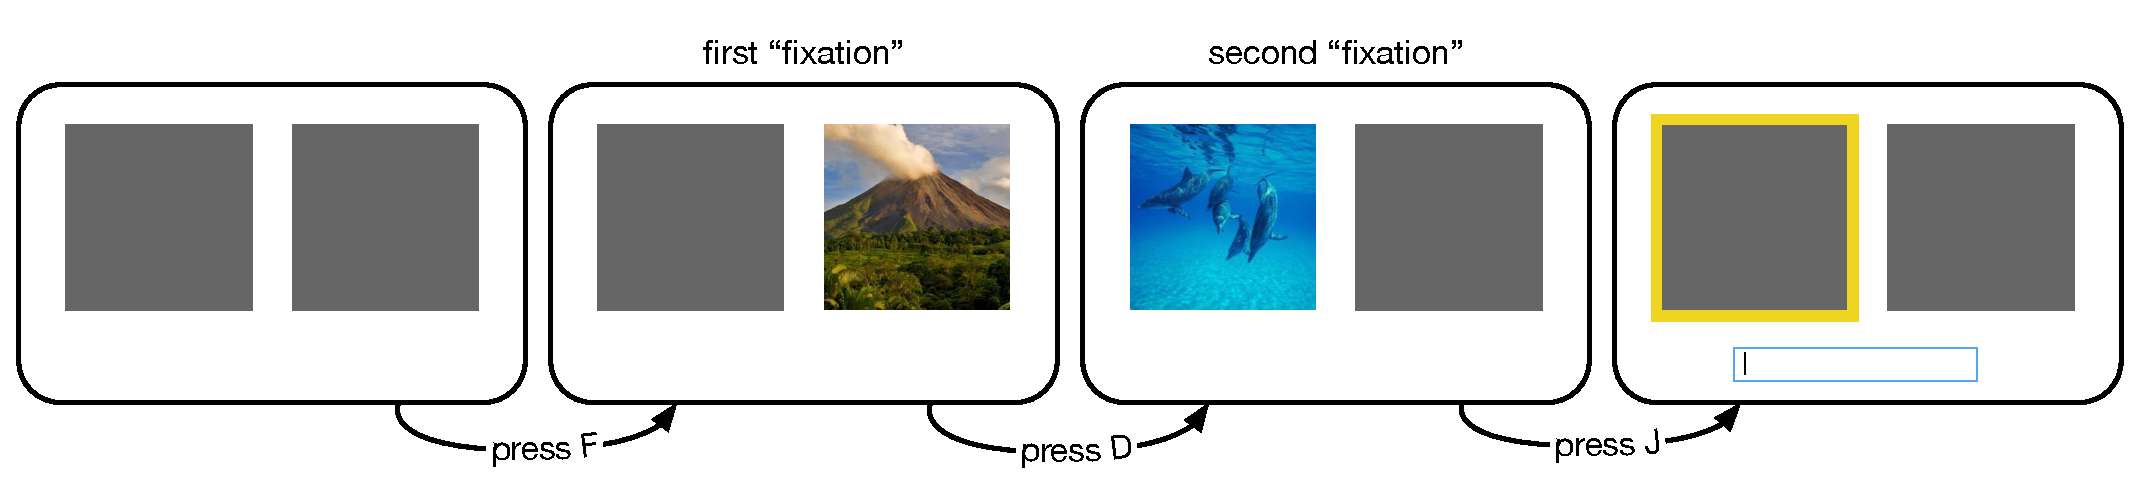
\includegraphics[width=\textwidth]{figs/memory/task_exp2.pdf}
  \caption{\captiontitle{Experiment 2 critical trials.} Participants were presented with two images on each trial and were instructed to recall the word associated with either of them. Only one cue was visible at a time and participant could flip between them with the D and F keys. At any point they could press J or K to select an image for recall, at which point they had five seconds to enter the associated word. We refer to the periods of time in which one cue was contiguously visible as ``fixations.''}
  \label{fig:task-exp2}
\end{figure}

\subsection{Discussion}

In this experiment, we found that participants were faster to recall targets with higher strength but slower to give up on targets with higher strength. Importantly, this pattern held for both a subjective measure of strength (replicating \citealp{costermans1992confidence}) as well as an objective measurement of strength (accuracy on the pretest trials). The latter is critical because it shows that people spent longer searching for memories that they were actually more likely to recall, thus demonstrating the objective utility of metamemory in guiding recall. Furthermore, because pretest accuracy is defined before the critical trials, this measure is not subject to the reverse-causality concern that response times are driving feeling of knowing rather than vice versa \citep{schwartz2001relation}. 

The full pattern of results was qualitatively consistent with the optimal model, which terminates search when the expected value of search falls below the expected cost, and reports a Bayesian estimate of strength as feeling of knowing or confidence. Perhaps more importantly, the results could \emph{not} be captured by a model without meta-level control. This provides computational support for the intuition that the correlation between search time and feeling of knowing is a distinctive signature of an adaptive metamemory process.

\section{Experiment 2}

In our first experiment, we considered a very simple form of metamemory, the decision of how long to search memory before giving up. Control of memory is not limited, however, to such a simple kind of decision. Instead, successful recall often requires deciding between multiple strategies for finding an answer \citep{reder1988strategic}. Going further, \citet{koriat2000control} has characterized recall as a form of problem solving, with a meta-level process ``coordinating between different operations directed toward the recovery of the elusive memory'' (p. 334). A careful characterization of the operations underlying recall (let alone how they are chosen) is beyond the scope of this paper. Nevertheless, in our second experiment, we sought to characterize a core aspect of this richer form of metamemory: monitoring multiple target memories and allocating retrieval efforts between them. 

On each trial, participants were presented with two cues and could recall the target for either one of them (Figure~\ref{fig:task-exp2}). They thus had to make a metacognitive decision about which of the two possible target to search for at each moment. In order to observe how this selection process unfolded over time, we used a keypress-contingent display, such that only one cue was visible at any moment. This provides process-tracing data similar to eye-tracking, but in a format amenable to online presentation.

\subsection{Predictions}

\begin{figure}[t!]
  \centering
  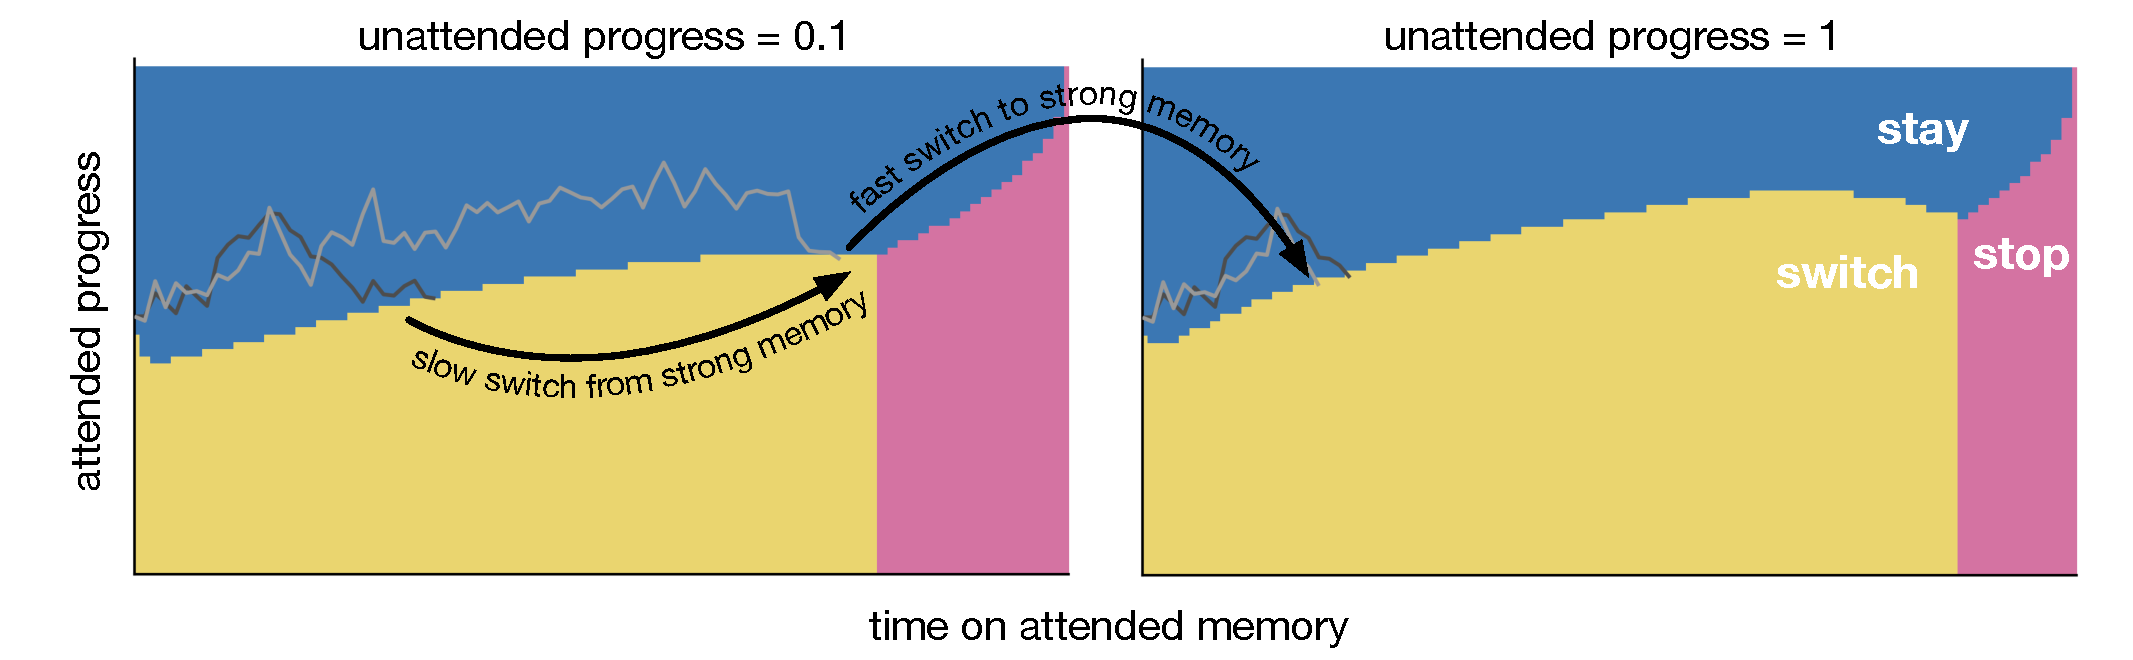
\includegraphics[width=\textwidth]{figs/memory/exp2_predictions.pdf}
  \caption{\captiontitle{Experiment 2 optimal policy and predictions.} With two possible memories to recall, the optimal policy partitions the state space into three sections where it is optimal to either: continue searching for the currently attended memory (blue), switch to the other memory (yellow) or give up (pink). The optimal policy depends on the recall progress and time spent on both memories; here we show two slices of the full four-dimensional state space, setting the time spent on the unattended memory to 10 timesteps and its progress to either 0.1 (left) or 1 (right). The gray lines show example progress traces for a weak (dark gray) and moderately strong (light gray) attended memory. The arrows highlight two key features of the optimal policy: it is less likely to switch when the currently attended memory is generating rapid progress, but more likely to switch if the unattended memory has already shown promise.}
  \label{fig:exp2_predictions}
\end{figure}

As detailed below, we extended the model to the multiple-memory case by creating a separate evidence accumulation process for each target memory. The meta-level process decides which accumulator is allowed to progress at each time point. The optimal policy (illustrated in Figure~\ref{fig:exp2_predictions}) can thus be characterized by when it decides to switch between the two memories (and also when it decides to terminate search, as before). 

In general, the optimal policy attends to the memory that it believes can be recalled soonest, as this will incur the least cost. In our experiment, attending to a memory is operationalized by looking at (or ``fixating'') the associated cue. Thus, the basic prediction is that the cues for stronger memories will receive a greater share of the total fixation time. More specifically, the model will be slower (and less likely) to switch away from a strong memory, but faster to switch when the other memory is strong.

Inspecting model simulations, we also discovered a surprising feature of the optimal policy. Its final fixations are longer than its non-final fixations. This prediction is surprising because we see the opposite pattern in decision-making tasks (e.g., \citealp{krajbich2010visual}, discussed further in the General Discussion). Why does the optimal policy make this prediction? We can understand long final fixations as sort of ``rational commitment'' behavior, in which the model effectively commits to recalling one memory before it is actually recalled. After committing to a memory, the model continues to attend to it until it is either recalled or its inferred strength drops well below the competitor. The latter occurs only rarely, thus the commitment tends to happen on final fixations, making those fixations longer. To see why this is rational, note that constant switching between the two memories is wasteful, as it can take up to twice as long as if one had immediately committed to one memory. On the other hand, immediately committing to the first cue could lead to getting stuck on an out-of-reach memory. Thus, the model only commits to a cue after becoming reasonably confident that the cue is strong.

We now describe an experiment that tests these predictions.

\subsection{Methods}

\subsubsection{Participants}

We recruited 685 participants through Prolific with the restriction that they reported current U.S. or U.K. residence, had at least a 95\% approval rating, and had not participated in any related studies (including pilots and Experiment 1). As pre-registered, we excluded 178 (26\%) participants who failed to correctly recall a target on more than 50\% of critical trials. This yielded 507 participants in our final analysis. The target sample size of 500 participants had over 95\% power based on a boot-strapping power analysis conducted on pilot data.

\subsubsection{Stimuli}

The stimuli were identical to those used in Experiment 1.

\subsubsection{Procedure}

The procedure was identical to Experiment 1 with two exceptions. First, we lengthened the training phase to include two blocks of exposure (with each cue/target pair shown once) and one intervening block of cued recall that was identical to the pretest block except that each pair was shown only once. Second, the critical trials followed an entirely different design described below.

\paragraph{Critical trials} The critical trials employed a modified form of cued recall in which two cues were presented on each trial. At the beginning of each trial, two gray occluders were displayed. Participants could temporarily remove the occluders, revealing the cue image underneath, by pressing the J and K keys. However, revealing one image would hide the other one. The 15-second timer appeared and began counting down when the first image was revealed. At any point, participants could press D or F to select one of the two cues for recall. At this point, both images were hidden, a yellow ring was drawn around the occluder for the selected image, and a text box appeared where they could enter the word associated with the selected image. Correct/incorrect feedback was provided after each response. Unlike Experiment~1, there was no penalty for errors (and hence, no skipping mechanism), no additional time incentive (besides the small incentive for fast correct answers that was also present in the pretest trials), and no collection of meta-memory judgments. Note that the lack of a skipping mechanism means that we cannot distinguish between genuine recall errors and the decision to give up on recall and enter a random guess (i.e., performing the $\term$ action). For this reason, we only analyze trials in which a target was correctly recalled. We decided to omit the skipping mechanism despite this drawback because we were specifically interested in the switching decisions (not the stopping decisions), and we wished to minimize task complexity.


\subsubsection{Modeling}

% \paragraph{Generalizing to multiple memories}

To generalize the model to the case with multiple memories that could be recalled, we assume that each memory is associated with its own independent object-level recall process. Furthermore, we assume that progress can be made on only one memory at a time, with the progress of the non-attended memory being held fixed. The state is defined $s_t = (t\cL, t\cR, z_t\cL, z_t\cR, f)$, with $t\cL$ and $t\cR$ denoting the number of timesteps the ``left'' and ``right'' memory have each been attended, $z_t\cL$ and $z_t\cR$ denoting their respective progress levels, and $f \in \{L, R\}$ indicating which memory is currently attended. When the progress for either memory hits the threshold, the corresponding target is recalled.

At the meta-level, the agent now has three actions: $\stay$, $\switch$, and $\term$. $\stay$ and $\switch$ are both similar to $\search$, but the latter additionally flips the value of $f$. We assume that there is some reconfiguration associated with switching. Thus the new reward function is:
%
\begin{equation}\label{eq:reward2}
  r(s_t, a_t) = \begin{cases} 
    U\recall & \text{ if } z_t \geq \theta \\
    -\samplecost & \text{ if } a_t = \stay \\
    -(\samplecost + \switchcost)  & \text{ if } a_t = \switch \\
    0 & \text{ if } a_t = \term.
  \end{cases}
\end{equation}

The new transition function has two parts. First, if the $\switch$ action is taken, $f$ is flipped. Then the original one-memory transition function is applied to the attended cue, updating the corresponding $t$ and $z_t$ variables. If the left memory is attended, we have
%
\begin{equation}\label{eq:mem-transition2}
  % T(s_{t+1} | s_t, a) = \int p(z_{t+1} \mid z_t, v)p(v \mid z_t, t) \ dv
  T(s_{t+1} | s_t, a) = p(z_{t+1}\cL \mid t\cL, z_t\cL)
\end{equation}
and similarly if the right cue is attended. We compute the optimal value function and policy by backwards induction as before. It is illustrated in Figure~\ref{fig:exp2_predictions}.


\paragraph{Computing the optimal policy}

We again computed the optimal policy by backwards induction. We applied the same discretization, and computed the transition function in the same way. Note that, because recall progresses for only one memory at a time, it is not necessary to represent the transition function over the full state space.

To compute the value functions, we began by initializing the value of terminal states to $U\recall$ if either recall progress exceeded the threshold and 0 if the combined time exceeded 150. We then computed the value at previous time steps by iterating backwards. In this case, for each time step, we must consider all combinations of time spent on each item that sum to the the time step under consideration. Additionally, we must consider three possible actions. Assuming the left cue is currently attended, the action values are
%
\begin{equation}
\begin{aligned}
  &Q^*(s, \search) = \\
    &\quad\sum_{z\cL_{t+1}} p(z\cL_{t+1} | t\cL, z\cL_t) 
    V^*(t\cL+1, t\cR, z\cL_{t+1}, z\cR_t, L) - \samplecost \\
  &Q^*(s, \switch) = \\
    &\quad\sum_{z\cR_{t+1}} p(z\cR_{t+1} | t\cR, z\cR_t) 
    V^*(t\cL, t\cR+1, z\cL_{t}, z\cR_{t+1}, R) - \samplecost - \switchcost\\
\end{aligned}
\end{equation}
%
with $Q^*(s, \term) = 0$ as before. Besides these differences, the procedure is identical to the one-memory case.

\paragraph{Parameter estimation}

Due to the high dimensionality of the data in this experiment (sequences of fixation durations), maximum likelihood estimation is computationally prohibitive. Although approximate fitting schemes are possible, given that we are not interested in the quantitative fit of the model, we instead used this as an opportunity to test the generalization capabilities of the model (c.f. \citealp{krajbich2011multialternative}). That is, we simply used the best-fitting parameters from Experiment~1. For the switch cost parameter, which was not present in the Experiment~1 model, we arbitrarily set $\switchcost = \samplecost$, noting that the predictions do not depend greatly on the exact value of this parameter. However, because the model must predict the duration of each fixation, the original non-decision time model is no longer appropriate. Instead, we assumed that non-decision time was added to each fixation independently. We fit the parameters of this model by maximizing the likelihood of all non-final fixation durations, assuming (for tractability) that they were independent and identically distributed. We excluded final fixations from this fitting procedure because they have different distributional properties (\figref{fig:commitment}{A}). The fitted NDT parameters were \(
            \mu_\text{NDT} = 611.72,\ 
            \alpha_\text{NDT} = 2.79
        \).


\begin{figure}[ht]
  \centering
  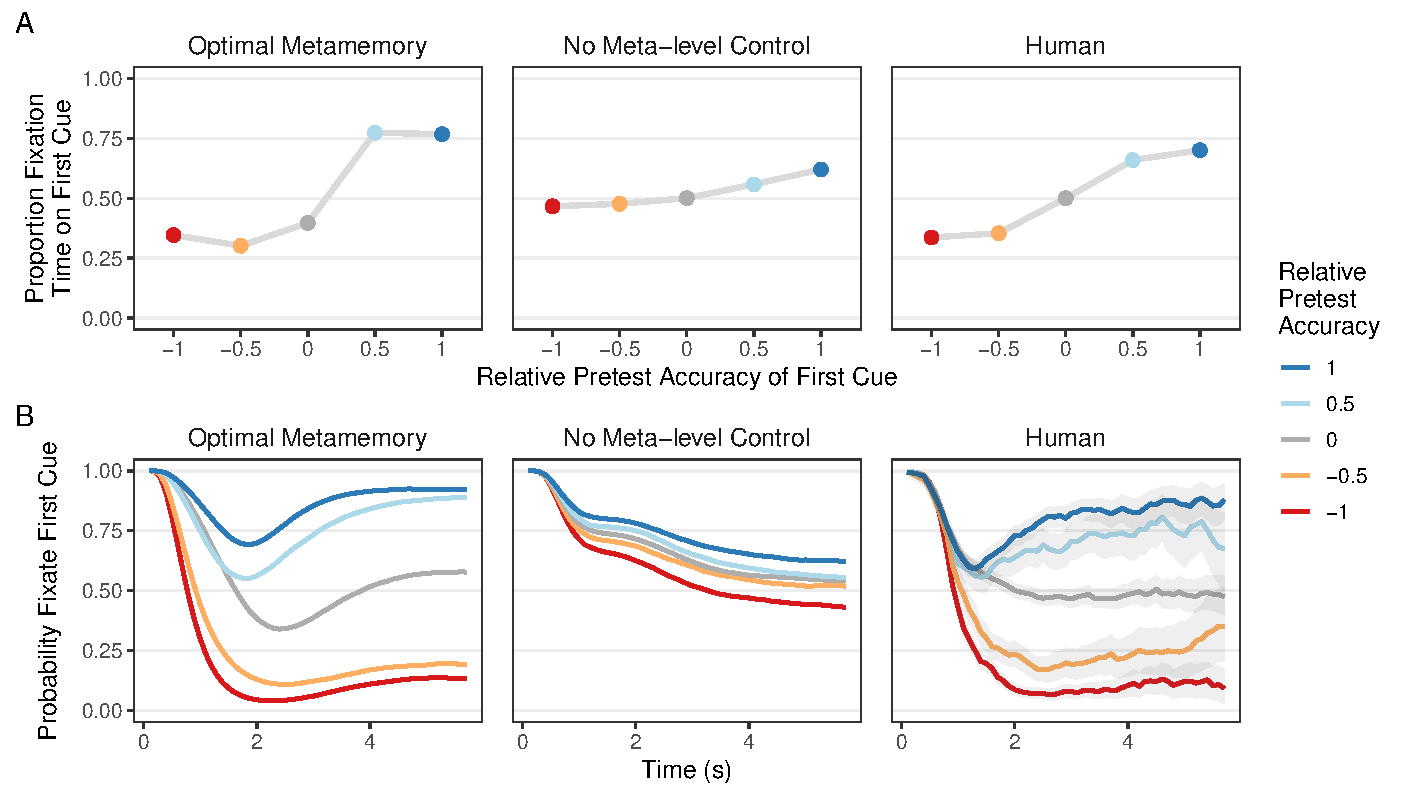
\includegraphics[scale=.65]{figs/memory/exp2/overall_timecourse.pdf}
  \caption{\captiontitle{Attention is drawn to stronger cues.}
    \subcap{A} The proportion of total viewing time allocated to the first-seen cue image as a function of the difference in pretest accuracy of the first- and second-seen cues. Trials for which the second cue was never shown are excluded. Note that the 95\% confidence intervals are too small to be distinguishable.
    \subcap{B} The probability that the first-seen cue is currently displayed over the course of the trial, split by relative pretest accuracy.
    % The x-axis extends to the 95\% quantile of response time.
  \label{fig:timecourse}
  }
\end{figure}

\begin{figure}[t]
  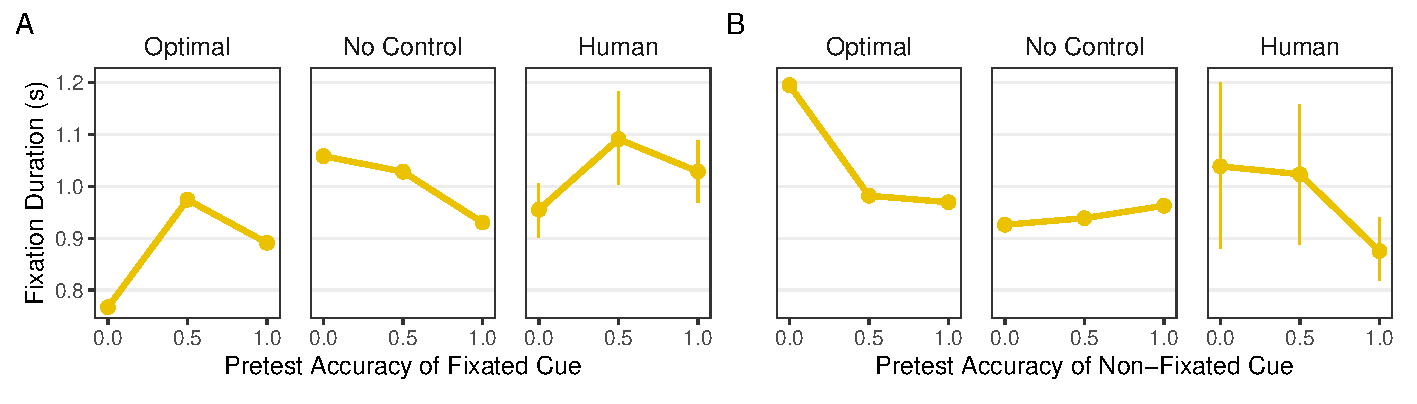
\includegraphics[scale=.65]{figs/memory/exp2/nonfinal.pdf}
  \caption{\captiontitle{Non-final fixation durations.}
    \subcap{A} The duration of non-final fixations as a function of the pretest accuracy of the currently fixated cue.
    \subcap{B} The same, but for the pretest accuracy of the cue that is \emph{not} currently fixated (first fixations excluded).
  \label{fig:nonfinal}
}
\end{figure}

\begin{figure}[t]
  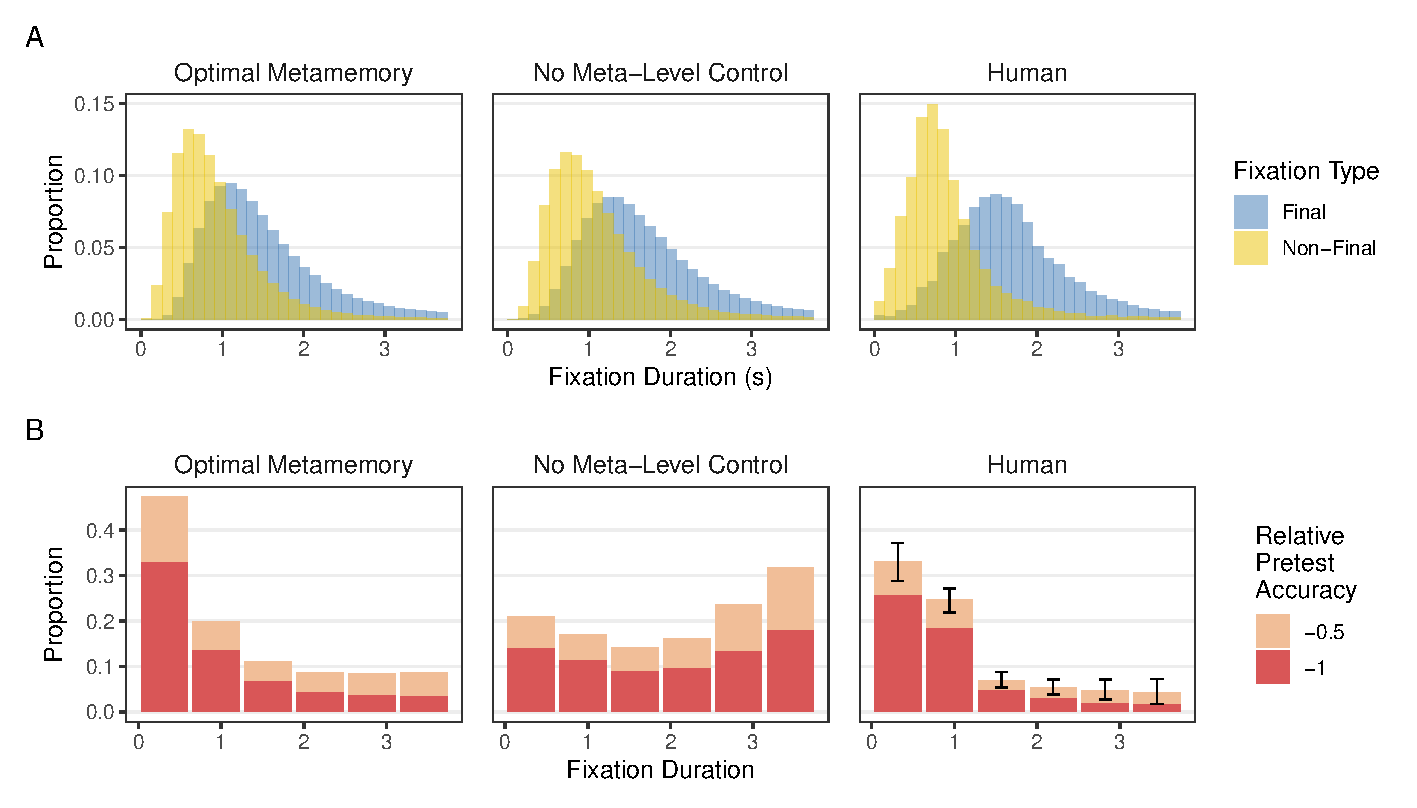
\includegraphics[scale=.65]{figs/memory/exp2/commitment.pdf}
  \caption{\captiontitle{Rational commitment to stronger cues.}
    \subcap{A} The distribution of final and non-final fixation durations.
    \subcap{B} The proportion of fixations on items with lower pretest accuracy than the alternative, separately for fixations of different durations (first fixations excluded). The error bars indicate 95\% confidence intervals computed over the total proportion (including -0.5 and -1) for each participant.
  \label{fig:commitment}
}
\end{figure}

\paragraph{Lesioned model without meta-level control}

The lesioned model is an extension of the lesioned model from Experiment~1, with an additional mechanism to determine fixation durations. As before, the stopping time was sampled from a Gamma distribution at the beginning of each trial. Similarly, at the beginning of each fixation, the switching time was sampled from a second Gamma distribution. If this time was reached before the memory was recalled or the stopping time was reached, then the model switched to attending the other cue and sampled a new switching time.

To give the lesioned model the best chance of capturing the qualitative effects, we fit all of its parameters to the behavioral data (in contrast to the Optimal model, which uses parameters fit to Experiment 1). Computing an exact likelihood is intractable in this case; thus, we approximated the likelihood by assuming that the duration of each fixation depends only on the pretest accuracy of the fixated and non-fixated cues, and whether or not the fixation is final. Given this assumption, we estimated the likelihood in the same way as for Experiment~1, with the exceptions that the histogram had size $3 \times 3 \times 2 \times 151$ (3 accuracy rates for each cue, final vs. non final, and 151 response time bins) and that the likelihood was computed per-fixation rather than per-trial. Note that we constructed the histogram using only correct simulated trials, as we exclude error trials from the human data. The MLE was (\(
            \mu_0 = 0.083,\ 
            \sigma_0 = 0.103,\ 
            \sigma = 0.148,\ 
            \mu_\text{stop} = 4527.0,\ 
            \alpha_\text{stop} = 76.16,\ 
            \mu_\text{switch} = 4943.0,\ 
            \alpha_\text{switch} = 0.18,\ 
            \mu_\text{NDT} = 810.0,\ 
            \alpha_\text{NDT} = 3.59,\ 
        \)).

\subsection{Results}

The critical model predictions concern participants' ``fixation'' behavior in the double-cued-recall trials, that is, the sequence of key presses they made to alternately display the two images. The most basic prediction of the optimal model is that participants should attend more to the cue with stronger memory. Intuitively, the target for the stronger cue can be recalled faster, and so time spent looking at this cue is more productive. Indeed, as illustrated in \figref{fig:timecourse}{A}, participants spent substantially more time looking at cues that were stronger than the other available cue ($B = 0.191$, 95\% CI [0.182, 0.199], $t(572.0)=42.40$, $p < .001$). However, this pattern is also shown (to a lesser extent) by a lesioned model that randomly switches between the cues. This is due to two properties of the object-level recall process. First, the last fixation is always on the cue whose target is recalled. Second, stronger cues are more likely to be recalled. Together, this implies that stronger cues are more likely to be fixated last, and thus receive more fixations (and more fixation time) on average.

Inspecting the timecourse of attention across the trial (\figref{fig:timecourse}{B}) reveals a more nuanced picture. People tend to quickly check both cues (as indicated by the the initial dip in probability of fixating the first cue). Then, if the second cue is stronger, they continue fixating it. But if the first cue is stronger, they switch back to it. From about one to three seconds, participants show an increasingly strong tendency to fixate the stronger cue, and this tendency remains stable for the remainder of the trial. The optimal model shows a similar pattern, although its tendency to fixate the stronger cue emerges faster (as indicated by the earlier divergence of fixation probability for different relative strengths). In the lesioned model, a slight tendency to fixate the stronger cue emerges in the first second, and remains small for the remainder of the trial.

Although the lesioned model was not able to capture the strength or timecourse of the tendency to fixate stronger cues, the fact that it can produce the effect at all casts some doubt on the interpretation of the pattern in human data. Thus, for our next analysis, we inspected the duration of individual non-final fixations, which are clearly not subject to the last-fixation confound. As illustrated in Figure~\ref{fig:exp2_predictions}, the optimal policy's decision to terminate a fixation by switching to the other cue depends on the recall progress of both targets; it is slower to switch when the currently attended cue is generating rapid progress, but faster to switch when the unattended cue has already generated substantial progress. The model thus predicts that non-final fixation durations will increase\footnote{%
    To be exact, the model predicts a non-monotonic effect such that fixations are longest for intermediate strength cues. This is due to the same selection effect that produces a non-monotonic prediction in \figref{fig:exp1_rt}{B}. Switching away from a strong cue suggests that the model incorrectly estimated its strength (because progress happened to be slow at first). This becomes increasingly unlikely as the fixation progresses and more evidence is collected. Such ``erroneous'' switches are thus more likely to occur quickly. 
} with the pretest accuracy of the fixated cue, but decrease with the pretest accuracy of the non-fixated cue. As illustrated in Figure~\ref{fig:nonfinal}, both of these predictions were confirmed: participants' non-final fixations increased with the pretest accuracy of the fixated cue ($B = 0.106$, 95\% CI [0.075, 0.137], $t(230.7)=6.65$, $p < .001$) and decreased with the pretest accuracy of the non-fixated cue ($B = -0.456$, 95\% CI [-0.578, -0.334], $t(59.7)=-7.32$, $p < .001$; first fixations excluded). The lesioned model predicts no such effect. In fact, it is incapable of predicting either effect under any parameter setting that achieves accuracy levels comparable to our participants (with very low accuracy, it can capture the effect through a selection mechanism; see Appendix~\ref{app:lesion-search}).\footnote{
    Again, the lesioned model predicts a reverse effect due to selection effects similar to those discussed in Experiment~1 and the previous footnote. For the fixated cue's strength, it is exactly the same logic as in Experiment~1. A strong cue is likely to be recalled quickly; it will only be switched away from when a short switching time is sampled. For the non-fixated cue's strength, the logic is more complex. Because we condition on one of the memories being recalled, the non-fixated cue being weak implies that the fixated cue is strong. Following the same logic as before, this in turn implies that a short switching time was sampled (as otherwise the cue would have been recalled).
}

For our final analysis, we tested the model's ``rational commitment'' behavior, in which the model effectively commits to recalling one memory before it is actually recalled. One observable consequence of this is that the model's final fixations are longer than their non-final fixations, as the commitment decision can occur when the memory is still well below threshold. Consistent with this, \figref{fig:commitment}{A} shows that our participants final fixations were indeed longer than their non-final fixations ($B = 0.872$, 95\% CI [0.813, 0.930], $t(435.9)=29.29$, $p < .001$). However, this figure also shows that the lesioned model can capture this effect as well. It is able to do this through a ``random commitment'' mechanism: by assuming a high-variance switching-time distribution, it occasionally samples a very long fixation duration, which is likely to end in recall. 

Did participants' long final fixations reflect rational commitment or random commitment? The key distinction between these types of commitment is that it is only rational to commit a memory that is at least as strong as the alternative. Thus, only with a random commitment strategy will one allocate long fixations to cues that are weaker than the alternative. \figref{fig:commitment}{B} thus shows the frequency with which the weaker memory is fixated, separately for fixations of different length. Importantly, we do not limit this analysis to final fixations as this would exclude the cases where the lesioned model sampled a long fixation duration on a low-strength cue, thus selecting for the cases where the lesioned model was ``accidentally'' rational. In both the optimal model and the human data, we see that long fixations are very unlikely to be directed to weaker memories. In contrast, under the lesioned model, the weaker cues are actually more likely to receive long fixations (because strong cues are likely to be recalled quickly, cutting off long fixations). The fact that people show a strong tendency to not direct long fixations to weak cues despite this selection effect suggests that their commitment decisions were indeed rational. Note, however, that we we did not pre-register this prediction because our initial, less flexible, implementation of the lesioned model that sampled switching times from the empirical distribution could not capture the long final fixation effect (see Appendix~\ref{app:deviation}, \figref{fig:commitment_alt}{A}). For this reason, we did not seek out further predictions to test the rational commitment mechanism. This result must thus be interpreted with some caution.

\subsection{Discussion}

In this experiment, we found evidence of a richer form of meta-level control of memory. Specifically, when presented with two cues associated with different target memories, our participants directed their attention towards the cue associated with the stronger memory. This was reflected in the overall proportion of fixation time, the timecourse of fixations, and the duration of individual non-final fixations. The latter two results are especially important because they are behavioral signatures of metacognitive control during the retrieval process itself (before recall is completed or abandoned). To our knowledge, this is the first empirical demonstration of a dynamic metamemory process unfolding over time. 

\section{General discussion}

In this paper, we presented an optimal model of meta-level control for cued recall. The model consists of a metacognitive process that monitors the progress of a basic recall process, and optimally controls how long the process is allowed to continue (either terminating recall or switching to recall of a different memory). In two experiments, we showed that human behavior is qualitatively consistent with the predictions of this model. In Experiment 1, we replicated and extended the findings of \citet{costermans1992confidence}, showing that people were faster to recall targets with higher strength (as indicated by both subjective judgments and objective performance) but slower to give up on targets with higher strength. In Experiment 2, we showed that people also attend to stronger memories when they can choose between two possible targets. Together, our results suggest that people can estimate the strength of a memory they are trying to recall and use this information to adaptively control their retrieval efforts.

\subsection{An explicit instantiation of a classic theory}

Our results contribute to the metamemory literature by providing (to our knowledge) the first computationally explicit instantiation of the classic theory of metamemory proposed by Nelson and Narens \citeyearpar{nelson1990metamemory} in the context of memory recall. According to this theory, metacognition involves the interaction between a meta-level process and an object-level process, where the meta-level process monitors the state of the object-level process and controls it accordingly. In the context of memory recall, they proposed a verbal model in which feeling of knowing is generated by ``an evaluation in terms of whether there has been sufficient progress to continue'', with the process terminating in an omission error when this feeling of knowing no longer ``exceeds the FOK threshold for claiming to know the answer'' (p. 137). They went on to suggest that this model could account for the correlation between feeling of knowing and response time on omission trials.

Here, we have formalized this classic model as a sequential decision problem in which the meta-level process executes a sequence of actions (continuing or terminating memory search) to maximize reward (utility of recall minus cost of search) given the observed state of the object-level process (recall progress). By formalizing this problem as an MDP, we could identify the optimal metacognitive control policy using standard dynamic programming techniques. This allowed us to generate quantitative predictions about the observable behavior we would expect to see if people were indeed using a rational metamemory system to control how long they search for an elusive memory. By confirming these predictions in an experiment, we have contributed quantitative support for this classic theory, which was previously supported only by intuitive qualitative predictions.

Formalizing Nelson and Naren's model as an MDP also allows us to create a conceptual link between metacognition and reinforcement learning (RL; \citealp{sutton2018reinforcement}). Specifically, we map the meta-level and object-level processes onto the concepts of agent and environment, respectively. That is, we model metacognition as a meta-level agent interacting with an object-level environment in much the same way as one would model, e.g., a mouse (the agent) searching for food in a maze (the environment). RL has become a major theoretical foundation in the psychology and neuroscience of decision-making \citep{niv2009reinforcement,dayan2008decision,glimcher2011understanding}. However, for the most part, it has been used to model the interaction between agents and \emph{external} environments. Applying RL to model the metacognitive interaction between an agent and its \emph{internal} environment (c.f. \citealp{simon1955behavioral}) creates the opportunity to transfer much of what we know about how people learn to act effectively in the world to understand how people learn to think effectively in their own minds \citep{lieder2018rational}.

\subsection{Rational analysis for metamemory}

Outside of metamemory, the intellectual roots of our model lie in Anderson's \citeyearpar{anderson1990adaptive} rational analysis, with early work demonstrating that the forgetting behavior commonly observed in lab settings is not a weakness or peculiarity of the memory system, but instead a reflection of rational adaptation to the statistics of the environment \citep{anderson1989human}. The key idea underlying both this models and ours is that memory (and cognition more generally) can be treated as an optimization problem. More recently, researchers have emphasized that this optimization problem must also account for the constraints imposed by our limited computational resources \citep{griffiths2015rational,howes2009rational,lewis2014computational,gershman2015computational}. This approach, sometimes called resource-rational analysis, has generated insight into a wide variety of cognitive processes (see \citealp{lieder2020resourcerational}, for a review).

Focusing on memory, a large body of work has shown that many apparent memory biases actually reflect optimal statistical reasoning under the constraint of noise or capacity limitations \citep{gershman2021rational}. For example, in reconstruction tasks, people draw on prior knowledge of a stimulus category to adjust for memory imprecision \citep{huttenlocher2000categories}, using more abstract categories for less familiar stimuli \citep{hemmer2009bayesian}. In working memory tasks, people are sensitive to cost-benefit trade-offs when choosing how many items to encode \citep{howes2016predicting}, how to allocate encoding resources across items \citep{yoo2018strategic}, and how much total resource to allocate \citep{vandenberg2018resourcerational}. Researchers have also begun to explore the implications of the constraints that emerge from more detailed models of memory. For example, \citet{zhang2022optimal} characterize the optimal order in which to recall items from a list, assuming that items are stored and recalled with the context maintenance and retrieval (CMR) model (\citealp{polyn2009context}; discussed further below). They find that the optimal policy is to start from the beginning of the list and then sequentially recall forwards, providing a rational account of the often-observed primacy and forward asymmetry effects \citep{zhang2022optimal}.

Focusing on metamemory in particular, two recent models of judgments of learning are based on signal detection theory \citep{jang2012stochastic} and Bayesian inference \citep{hu2021bayesian}, both of which have rational bases in probability theory. However, these models only attempt to explain how metamemory judgments are produced, not how they are used---a critical component in a complete rational analysis. We are aware of two computational models that explicitly address the function of metamemory judgments and both take an explicitly rational approach. \citet{hu2019role} proposed a model of cognitive offloading, in which a rational agent decides whether or not to use an external memory aid by comparing the expected increase in recall probability with the reduction in payoff. Most similar to our own work, \citet{suchow2016deciding} proposed an MDP model of working memory maintenance, in which an agent selects actions that increase the strengths of different memories, as encoded in the state. This model could account for the findings of \citet{williams2013benefit}, in which directing participants to forget certain items reduced recall accuracy for the cued item and increased accuracy for uncued items.

Our model draws on several specific ideas from the work described above, in addition to the core principle of rationality. Like \citet{anderson1989human}, we frame the decision to terminate search as a cost-benefit comparison (Equations~\ref{eq:anderson} and~\ref{eq:policy}). Like \citet{vandenberg2018resourcerational}, we jointly consider the problem of how much resource to allocate (here, the resource being time) as well as how to split that resource between items. Like \citet{hu2021bayesian}, we model metamemory judgments as the product of Bayesian inference about the strength of a memory. And like \citet{suchow2016deciding}, we model the resource allocation problem as an MDP. Our work contributes to this literature by synthesizing these previous insights, and showing how they can be applied in a new domain, cued recall.

Importantly, like the other resource-rational models reviewed above, our model aims only to characterize the optimal solution to the problem of cognition under limited resources. We have not attempted to explain how the mind might actually approximate that solution. We do note, however, that executing the optimal policy for our model does not require one to continually perform Bayesian inference over the memory strength. Indeed, as illustrated in Figure~\ref{fig:exp1_predictions}, the optimal policy in the one-cue case is defined by a single boundary, such that recall is terminated if the evidence ever falls below it. Although we identified the shape of this optimal boundary with computationally intensive, model-based methods, it could be well-approximated by simple model-free learning mechanisms. Understanding how people learn effective metacognitive strategies is a subject of ongoing research \citep{lieder2018rational,jain2019how,callaway2022leveraging,binz2022heuristics,he2022where}.

\subsection{Imperfect monitoring and cue familiarity}
While our results make a strong case for the existence of an adaptive metamemory control system in the human mind, we do not claim to have characterized the precise nature of this system. Indeed, for simplicity and tractability, we made several assumptions that are most likely inaccurate. 
% For example, the distribution of memory strength is likely not exactly Gaussian and the true dynamics of recall progress are only coarsely described by a Brownian diffusion process (likely having a more staltory structure).
Perhaps most critically, we assumed that the meta-level process has direct access to the state of the object-level process (the recall progress). This form of monitoring can be seen as a simplified form of Koriat's \citeyearpar{koriat1993how} accessibility model. Specifically, our simplification does not allow for the possibility that incorrect partial information is recalled, which eliminates any divergence between feeling of knowing and recall progress. While this assumption greatly simplified the implementation of the model and has precedence in previous metamemory models \citep{suchow2016deciding,hu2019role}, perfect monitoring is intuitively implausible and it is inconsistent with the sensitivity of feeling-of-knowing judgments to spurious information generated during recall \citep{koriat1993how} and manipulations that do not affect accuracy (discussed below).

Beyond imperfect monitoring of recall progress, the meta-level process could rely on other sources of information about a memory's strength. An influential such theory suggests that feeling-of-knowing judgments are based on \emph{cue familiarity}, that is, the degree to which one feels that they recognize the prompt or question that triggered the memory search \citep{metcalfe1993cuefamiliarity}. Much evidence supports this view. For example, participants give higher feeling-of-knowing judgments to arithmetic problems that visually resemble previously seen problems \citep{reder1992determines}. Similarly, priming words in a question increases feeling-of-knowing without increasing recall \citep{reder1987strategy,reder1988strategic,schwartz1992cue}. Indeed, this fact, along with the observation that priming the memory target does not increase feeling of knowing, has led some researchers to suggest that feeling of knowing does not depend at all on partial recall (\citealp{reder1992determines,schwartz1992cue}; but c.f., \citealp{jameson1990influence,narens1994subthreshold}). On the other hand, the observation that people in tip-of-tongue states are able to correctly recall some aspects of the memory target, such as the number of syllables \citep{brown1966tip} or semantic associations \citep{koriat1993how,schacter1985attribute} suggests that partial recall may influence metamemory, although perhaps only in later stages of the recall process (c.f., \citealp{nhouyvanisvong1998rapid}).

It is thus plausible that metamemory draws on both partial recall progress and other factors such as cue familiarity. Indeed, this possibility has been formalized and supported by models in which a meta-level and object-level signal are imperfectly correlated \citep{fleming2017selfevaluation,jang2012stochastic,hu2021bayesian}. Intuitively, the meta-level signal in these models contains some information about recall progress (or ``processing experience'') and some information about the underlying memory strength from other sources (e.g. cue familiarity), with both components corrupted by independent noise. Our model can be seen as a special case of this class of models, where the amount of information from other sources and the noise are both fixed to zero. Allowing the noise to be non-zero would result in a formalization of Koriat's \citeyearpar{koriat1993how} accessibility model, in which metamemory is a noisy readout of actual recall progress. Further allowing additional sources of information besides recall would yield a complete model in which control is jointly informed by recall progress and ancillary cues. Unfortunately, both of these generalizations make the meta-level belief state depend on the full trajectory of signals (as opposed to just the sum), making the optimal policy intractable to solve.\footnote{%
  To see why this is, note that when the recall progress is not directly observed, the agent must infer a posterior distribution over it. This posterior must account for the continual observation that the boundary has not been crossed, and the likelihood of that event depends on the order of the signals. For example, if a large positive signal is followed by a large negative signal, the fact that the threshold was not crossed after the first signal indicates that the large positive signal was not accompanied by a similarly large change in progress. If the order is reversed, no such inference is drawn, and so the estimated recall progress across the two time steps will be higher.
} Nevertheless, exploring the implications of imperfect monitoring and cue familiarity for meta-level control (with suitable approximations to the optimal policy) is a critical direction for future research.

Finally, we emphasize that our we do not take our empirical results to support any specific theory of monitoring. Although we have only implemented a model that monitors partial recall, we believe that similar predictions could be made by a model whose monitoring component is based purely on cue familiarity. For this reason, we have taken care not to claim that our results suggest that people can monitor the progress of memory recall. Our results simply suggest that people are capable of inferring the \emph{strength} of a memory. Rigorously evaluating computational models of exactly how people make that inference will require additional data. Developing a paradigm to produce that data is another critical direction for future research.

\subsection{Beyond cued recall}

Although we have focused on cued recall, the decision about when to terminate search is present in almost all naturalistic recall tasks, including, for example, free recall. The basic principle of our model is that this decision should be made by balancing the benefit and probability of recall with the cost of search, a principle we inherit from \citet{anderson1989human}. This is in contrast to existing models of free recall such as the context maintenance and retrieval (CMR) model, which assumes that search is terminated either when a target memory is retrieved or after a fixed amount of time has passed \citep{polyn2009context,lohnas2015expanding}. Alternatively, according to the Search of Associative Memory (SAM) model, search is terminated after a fixed number of retrieval attempts that do not result in recall of a new word \citep{raaijmakers1981search}. In both models, the decision to terminate recall is based on a general stopping rule independent of the state of the memory system. Integrating a rational metacognitive stopping rule into these models is an interesting direction for future research. Empirically validating such a model will likely require additional data, as participants in free recall experiments are typically given a fixed amount of time to recall as many items as possible; the decision to terminate search cannot be observed in this setting.

% Our model could be extended to free recall by embedding it into a model such as CMR. CMR captures dynamics of free recall by assuming that items are associated with a context space during encoding and later retrieved given contextual cues at recall. As more items have already been successfully recalled from the context space, it becomes increasingly difficult to recall from the remaining items because the context space is being depleted. If there is metamemory to monitor how depleted the space is, we can imagine a CMR with a termination rule that is similar to our proposed model that balances the benefit and probability of recall with the cost of search. Such a model could explain \citeauthor{miller2012recall}'s finding that the duration between the last successful retrieval and the termination response (``exit latency'') decreased as the total number of items recalled increased \citep{miller2012recall}, as continuing the search becomes less likely with decreased probability of recall. A model such as the one sketched above would account for this, and thus be faster to terminate recall. This would explained the observed reduction in exit latency.

Metamemory goes beyond simply deciding when to terminate search. In Experiment~2, we considered the problem of arbitrating between multiple externally provided memory cues. In more naturalistic settings, however, people may need to generate their own cues. Indeed, in some cases, people generate information that is incidental to the information they are searching memory for, for example, recalling where people live in an attempt to recall their names \citep{williams1981process}. These incidental pieces of information can then be used as ``stepping stones on the way to the sought-after target'' \citep[p. 334]{koriat2000control}. This metaphor highlights the sense in which memory recall is a sequential decision problem. In our framework, each generated cue would correspond to a meta-level action, with some actions serving only to bring one to a mental state where one can generate a more useful cue. This suggests a fascinating direction for further research: How do people know which ``stones'' are going in the right direction?

\subsection{Beyond memory}

Our results also contribute to the literature on metacognition more broadly. Beyond memory, a wide variety of functional roles for metacognition have been proposed, including the regulation of perception \citep{deroy2016metacognition}, judgment \citep{polania2019efficient,lebreton2015automatic}, decision-making \citep{yeung2012metacognition,demartino2013confidence}, learning \citep{fromer2021expectations,nassar2012rational}, information seeking \citep{boldt2019confidence,desender2018subjective}, and social interaction \citep{frith2012role}. Some of these roles have been incorporated into computational models that formally describe how confidence might inform decision about, e.g., when to opt out of a difficult trial \citep{kiani2009representation}, when to change one's mind given additional evidence \citep{folke2016explicit}, how to interpret error feedback \citep{fromer2021expectations}, or where to fixate in visual search \citep{stewart2022humans}. However, these models often assume that the functional role of metacognition is \emph{static}. Although the mechanism underlying confidence judgments may be dynamic (typically being based on evidence accumulation \citealp{vickers1970evidence,pleskac2010twostage,moreno-bote2010decision}), any resulting metacognitive control occurs in a separate stage, typically as a single action, and not feeding back onto the object-level process in a dynamic, interleaved way. In an influential review, \citet{yeung2012metacognition} identified this as a critical gap to be explored in future research.

In the intervening decade, this gap has already begun to be filled. In particular, a substantial body of work has explored the within-trial dynamics of metacognition in controlling a decision-making process. These models track posterior distributions over an evidence accumulation rate and use this information to make optimal decisions about when to stop accumulating evidence \citep{drugowitsch2012cost,woodford2014stochastic,bitzer2014perceptual,fudenberg2018speed,tajima2019optimal} or how to allocate attention between multiple options \citep{jang2021optimal,callaway2021fixation}. However, to our knowledge, this type of model has been applied exclusively in decision-making contexts. Here, we have shown how a model with very similar structure can be applied to memory recall. 

The key structural difference between the model proposed here and these previous models of dynamic metacognition for decision-making is the assumption of an \emph{exogenous} threshold associated with recall. That is, the amount of ``evidence'' necessary to recall a memory is not under the agent's control. This contrasts with decision-making models, where both thresholds (for choosing each option) are \emph{endogenous}. The agent can choose an option based on very little evidence if they so desire. This simple change has a profound effect on the role of attention in the model. In the decision-making context, the sole purpose of fixating an option is to collect information about its utility. In the memory context, fixating the cue similarly provides information about its strength; but it also contributes to recalling the associated memory. 

This additional functional role for attention (stimulating recall as well as estimating strength) has two important consequences for the model's predictions in the two-memory case. First, the model predicts---and our results confirm---that cues for stronger memories receive more fixation time. In contrast, optimal models of attention in binary choice predict equal attention to high- and low-value items \citep{callaway2021fixation,jang2021optimal,fudenberg2018speed}.
% , a prediction that is sometimes supported by data.\footnote{%
%     In value-based choice, \citet{krajbich2010visual} report little to no effect of value on fixation durations. However, in a perceptual choice task, \citet{tavares2017attentional} find a moderate effect.
% } 
Second, the model predicts---and again, our results confirm---that final fixations are longer than non-final fixations. In contrast, evidence accumulation models of attention-guided decision-making predict that final fixations will be shorter than non-final fixations, a prediction that is consistently confirmed in data \citep{krajbich2010visual,krajbich2011multialternative,tavares2017attentional}. The fact that such a simple structural change can account for these major qualitative differences in the allocation of attention in value-based choice vs. cued recall suggests the promise of our MDP-based approach as a general framework for modeling metacognition.


\subsection{Conclusion}

In this paper, we have developed and experimentally validated a model of optimal meta-level control for memory recall. This model can be seen as a union of three influential frameworks in cognitive science: rational analysis \citep{anderson1990adaptive}, the two-process model of metacognition \citepnelson{}, and reinforcement learning \citep{dayan2008decision}. Concretely, we characterized a rational metamemory system as the optimal policy for a Markov decision process in which a meta-level agent monitors and controls its object-level environment in order to maximize reward. Although here we have focused on metamemory, we are optimistic that this approach could be applied to model metacognition in other domains as well. We believe that dynamic metacognitive processes such as the one studied here are a critical, but understudied feature of human cognition. We thus hope that our work will encourage other researchers to further develop a rich, computational understanding of these important processes.


\subsection*{Acknowledgments}
This research was supported by a grant from Facebook Reality Labs.
